% \documentclass[letterpaper, conference, 10pt]{IEEEtran}

\documentclass[10pt,journal,compsoc]{IEEEtran}

\ifCLASSINFOpdf
\else
 \fi

\newcommand\inlineeqno{\stepcounter{equation}\ (\theequation)}
% \usepackage{caption}
% \usepackage{subcaption}
% \usepackage{lipsum,multicol}
\usepackage[T1]{fontenc}
\usepackage{booktabs}
\usepackage[ruled,vlined,linesnumbered]{algorithm2e}
\usepackage{amsthm}
\usepackage{amsmath}
\usepackage{graphicx}
\usepackage[compatible]{algpseudocode}
\usepackage{amssymb}
\usepackage{amsfonts}
\usepackage{algcompatible}
\usepackage{tabularx}
\usepackage{lipsum}
\DeclareMathOperator*{\maxi}{maximize}
\DeclareMathOperator*{\argmax}{arg\,max}
\DeclareMathOperator*{\argmin}{arg\,min}
\usepackage[utf8]{inputenc}
\newtheorem{theorem}{Theorem}
\newtheorem{defn}{Definition}
\newtheorem{lem}{Lemma}
\usepackage{url}
\usepackage{xcolor}
%\usepackage{cite}
\usepackage{balance}
\usepackage{subcaption}
\usepackage{epstopdf}
\usepackage{array}
\usepackage{comment}
\usepackage[noadjust]{cite}
\usepackage{tipa}
\usepackage{breqn}
\newtheorem{claim}{Claim}
\newtheorem{lemma}{Lemma}
\SetKw{Continue}{continue}
\SetKw{Break}{break}
\SetKwFor{RepTimes}{repeat}{times}{end}
\usepackage{mathtools}
\DeclarePairedDelimiter\ceil{\lceil}{\rceil}
\DeclarePairedDelimiter\floor{\lfloor}{\rfloor}



% \usepackage{tikz}
% \usetikzlibrary{matrix,shapes,arrows,positioning,chains,backgrounds}
\newtheorem{corollary}{Corollary}
\usepackage[usestackEOL]{stackengine}
\usepackage{multirow}
\usepackage{makecell}

\hyphenation{op-tical net-works semi-conduc-tor}


\begin{document}

\title{AI-driven Continuous Network Slicing for HealthCare}



\author{Moirangthem Biken Singh and Pradeep Kumar Saran, ~\IEEEmembership{Member,~IEEE}
	\IEEEcompsocitemizethanks{\IEEEcompsocthanksitem M. B. Singh, N. Taunk, N. K. Mall and A. Pratap are with the Department of Computer Science and Engineering, Indian Institute of Technology (Banaras Hindu University), Varanasi 221005 India. E-mail: \{moirangthembsingh.rs.cse21, navneettaunk.cse18, naveenkumarmall.cse18, ajay.cse\}@iitbhu.ac.in.\protect 
    	 }
	}




\IEEEtitleabstractindextext{%
\begin{abstract}
The rapid growth of smart healthcare systems has enabled continuous patient monitoring through Internet of Things (IoT) enabled medical devices, wearable sensors, and Wireless Body Area Network (WBAN) based healthcare applications. However, critical healthcare services such as ambulance communication, ICU monitoring, emergency response systems, telemedicine, and remote patient monitoring require ultra-low latency, high reliability, efficient bandwidth utilization, and energy-aware communication over 5G networks. Conventional static network slicing approaches are insufficient to handle continuously varying healthcare traffic demands and dynamic network conditions, often leading to inefficient resource utilization and degradation in Quality of Service (QoS) for latency-sensitive medical applications.

To address these challenges, this work proposes an AI-driven framework for continuous network slicing and intelligent resource allocation in smart healthcare systems over 5G networks. The proposed architecture integrates edge computing with machine learning techniques, where Long Short-Term Memory (LSTM) is employed for healthcare traffic prediction, emergency-aware traffic classification is used to identify critical medical conditions, and Deep Deterministic Policy Gradient (DDPG) based deep reinforcement learning is utilized for continuous bandwidth allocation and adaptive resource optimization. The framework continuously monitors network conditions and dynamically adjusts slice configurations and resource distribution according to healthcare traffic demand, emergency level, and service priority requirements.

A multi-objective optimization model is developed by jointly considering end-to-end latency, reliability, throughput, power consumption, and resource energy utilization as key performance metrics. The latency model incorporates transmission delay, queueing delay, edge processing delay, AI decision delay, and slice adaptation delay to capture real-time communication performance. The objective is to minimize communication latency and power consumption while maximizing throughput, reliability, and energy-efficient resource utilization for latency-sensitive healthcare services. Experimental evaluation demonstrates that the proposed framework significantly improves adaptive resource allocation efficiency, reduces communication delay, enhances network reliability, and provides an efficient intelligent communication framework for next-generation 5G-enabled smart healthcare systems.
\end{abstract}
\begin{IEEEkeywords}
5G Networks, Smart Healthcare, Continuous Network Slicing, Deep Reinforcement Learning, DDPG, LSTM, Edge Computing, Resource Allocation, Latency Optimization, Reliability, Throughput, Energy Efficiency.
 
\end{IEEEkeywords}}

\maketitle

\IEEEdisplaynontitleabstractindextext

\IEEEpeerreviewmaketitle
   

\IEEEraisesectionheading{\section{Introduction}\label{sec:introduction}}

The rapid advancement of Internet of Things (IoT) based healthcare systems has enabled continuous patient monitoring through wearable sensors, Wireless Body Area Networks (WBAN), and real-time healthcare applications. With the emergence of 5G communication networks, healthcare services such as ambulance communication, ICU monitoring, telemedicine, and remote patient monitoring have become increasingly dependent on reliable and low-latency communication systems \cite{zhai2021ambulance}. The high bandwidth availability, ultra-low latency, and massive connectivity offered by 5G make it suitable for supporting next-generation smart healthcare applications.

However, healthcare communication systems are highly latency-sensitive and require efficient resource management to handle dynamic and heterogeneous traffic generated by multiple connected medical devices. Critical healthcare services such as emergency response systems and ICU monitoring demand immediate network access and uninterrupted communication. Traditional static network slicing approaches allocate fixed resources and often fail to adapt efficiently to continuously changing traffic conditions, resulting in network congestion, inefficient bandwidth utilization, and degradation in Quality of Service (QoS).

Continuous network slicing has emerged as an effective solution for dynamically adapting network resources according to real-time service requirements. In addition, edge computing helps reduce communication delay by processing healthcare data closer to end devices rather than relying entirely on cloud infrastructure. Recent advances in Artificial Intelligence (AI) and Deep Reinforcement Learning (DRL) enable intelligent optimization of such dynamic network environments. Machine learning models such as Long Short-Term Memory (LSTM) can predict future traffic demand, while Deep Deterministic Policy Gradient (DDPG) can continuously allocate bandwidth and optimize resource utilization. The overall proposed architecture of the AI-driven healthcare communication framework is shown in Fig. \ref{model}.

\begin{figure}[!t]
\centering
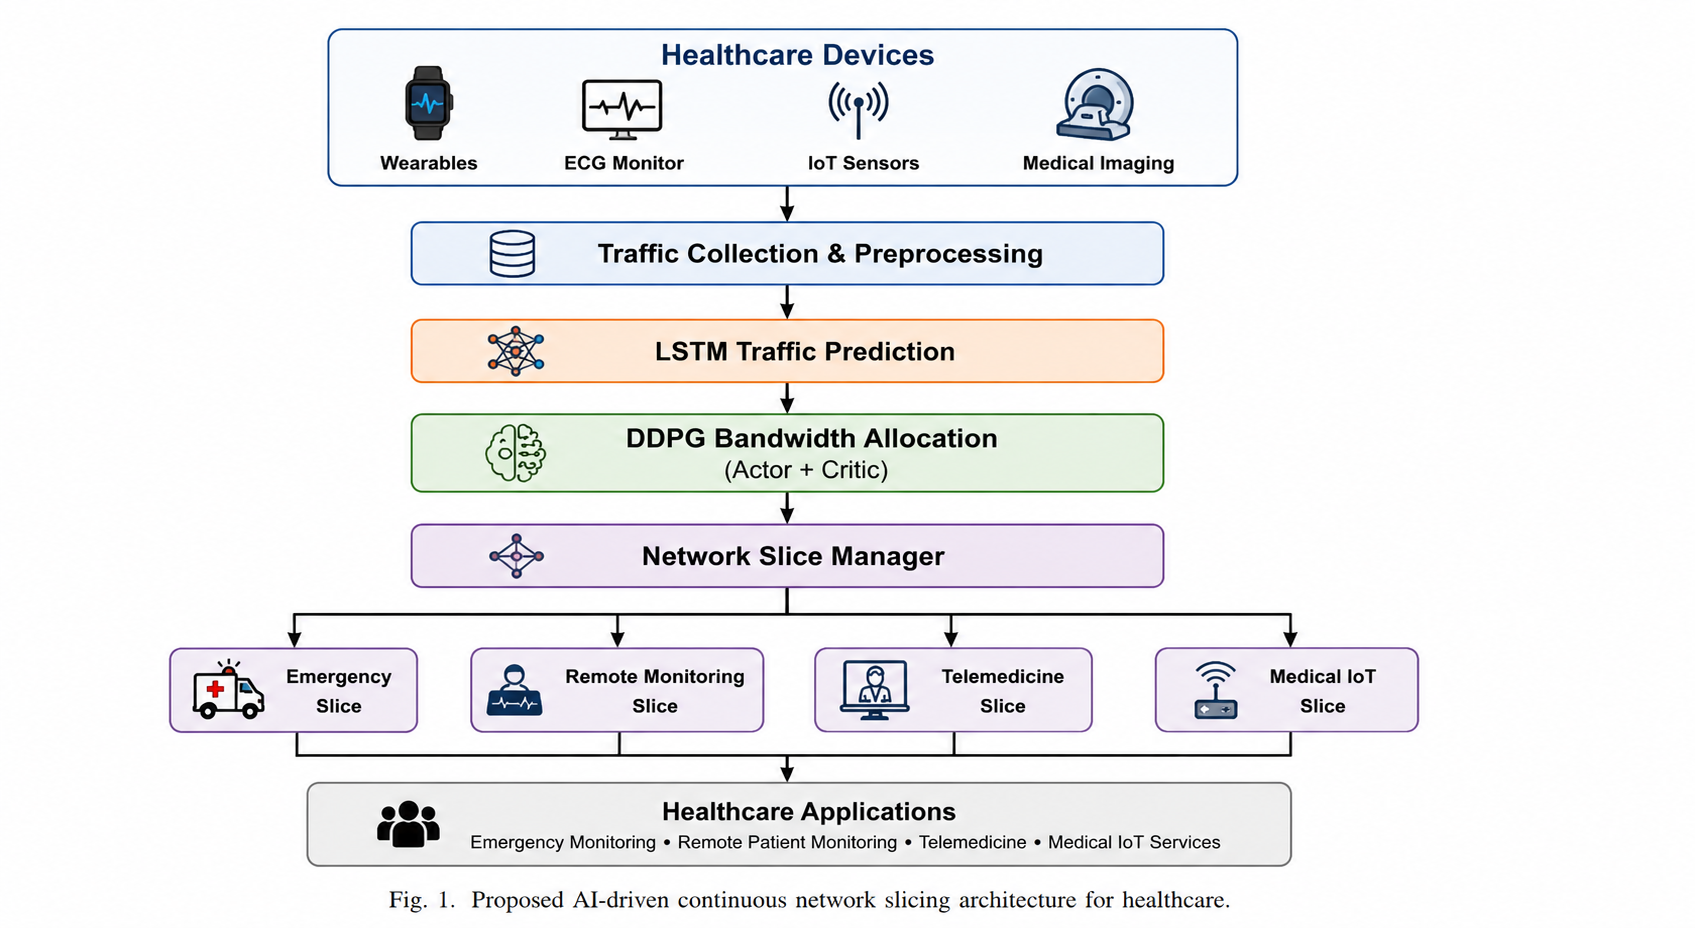
\includegraphics[width=8cm,height=4.8cm]{architecture.png}
\caption{Proposed AI-driven continuous network slicing and resource allocation architecture for smart healthcare over 5G networks.}
\label{model}
\end{figure}

Motivated by these challenges, this work proposes an AI-driven framework for continuous network slicing and intelligent resource allocation for smart healthcare systems over 5G networks. The proposed system integrates healthcare IoT devices, edge computing, machine learning intelligence, and adaptive slicing mechanisms to improve communication efficiency for real-time healthcare applications.

In nutshell, contributions of this paper are summarized as below:

\begin{itemize}

\item Propose an AI-driven smart healthcare architecture over 5G networks integrating IoT healthcare devices, edge computing, and continuous network slicing.

\item Employ LSTM based traffic prediction and emergency-aware healthcare traffic classification for intelligent network management.

\item Utilize DDPG based deep reinforcement learning for continuous bandwidth allocation and adaptive resource optimization.

\item Formulate a multi-objective optimization framework considering latency, throughput, reliability, power consumption, and resource energy utilization.

\end{itemize}

The rest of the paper is organized as follows: Section II reviews related work. Section III presents the system model and problem formulation. Section IV describes the proposed framework. Section V presents performance evaluation. Finally, Section VI concludes the paper and discusses future work.







\section{Related Works}\label{SecII}

This section presents closely related works available in the literature with comparative analysis as shown in Table \ref{related_works}.

Several existing works have focused on improving communication efficiency and resource management in 5G enabled smart healthcare systems. Authors in \cite{basu2022softhealth} primarily focused on healthcare communication over 5G networks while improving Quality of Service (QoS) and enabling real-time healthcare applications using machine learning assisted network slicing. In \cite{wijethilaka2022hospital}, the authors presented a comprehensive analysis of network slicing architectures for smart hospital applications in next generation healthcare systems. Similarly, authors of \cite{yaqoob2026aqps} focused on adaptive QoS-aware priority scheduling and dynamic radio resource allocation in multiservice 5G network slicing environments. However, these works mainly focused on communication performance and did not consider intelligent continuous network slicing under dynamically changing healthcare traffic conditions \cite{gollavilli2024healthcare}.

Recent research has shown significant progress in applying Artificial Intelligence and Machine Learning techniques for network optimization in dynamic communication systems \cite{hurtado2022drlsurvey,dubey2024ai,helmy2025slicing}. In \cite{kumar2025lstmddpg}, the authors proposed an attention based LSTM-DDPG framework for traffic prediction and efficient resource allocation in beyond 5G network slicing environments. Authors in \cite{saleh2025hybridrl,narode2025resource,yu2026dynamic} utilized hybrid reinforcement learning for intelligent resource allocation and bandwidth optimization in 5G network slicing systems. Similarly, \cite{tariq2025ddpgv2x,yang2025ddpg} proposed DDPG based resource management for dynamic resource allocation in 5G advanced service environments. However, these approaches did not specifically consider healthcare traffic criticality, emergency-aware communication prioritization, and continuous slice adaptation under heterogeneous healthcare service requirements.

Several works have also investigated network slicing mechanisms for heterogeneous 5G services \cite{wijethilaka2021iotslicing}. The authors in \cite{shah2025oran,ari2025iot5g,zhang2026trustaware} proposed dynamic AI-driven network slicing frameworks with O-RAN architecture for continuous connectivity and adaptive service management in next generation wireless systems. In \cite{zheng2025eamem}, the authors focused on adaptive network slicing and hierarchical resource management using edge assisted architectures for dynamic service optimization. Authors of \cite{sarker2026prioritybw} proposed priority based bandwidth allocation mechanisms for network slicing enabled wireless communication systems. However, most of these works rely on static or semi-dynamic slicing approaches and do not address continuous slicing, emergency-aware healthcare traffic prioritization, and energy-efficient resource utilization for real-time smart healthcare applications \cite{sun2025xai6g}.



\begin{table}[!t]
\begin{center}
\caption{Comparative analysis of existing approaches}
\label{related_works}

\begin{tabular}{| c | c | c | c | c | c |}
\hline

\textbf{\Centerstack{Existing\\Work}} &
\textbf{\Centerstack{Health-\\care}} &
\textbf{\Centerstack{Continuous\\Slicing}} &
\textbf{\Centerstack{AI/ML\\Based}} &
\textbf{\Centerstack{DRL\\Based}} &
\textbf{\Centerstack{Multi-\\Objective}} \\

\hline

\Centerstack{\cite{basu2022softhealth}} &
\checkmark &
$\times$ &
\checkmark &
$\times$ &
\checkmark \\

\hline

\Centerstack{\cite{wijethilaka2022hospital}} &
\checkmark &
$\times$ &
$\times$ &
$\times$ &
\checkmark \\

\hline

\Centerstack{\cite{yaqoob2026aqps}} &
$\times$ &
\checkmark &
$\times$ &
$\times$ &
\checkmark \\

\hline

\Centerstack{\cite{kumar2025lstmddpg}} &
$\times$ &
\checkmark &
\checkmark &
\checkmark &
\checkmark \\

\hline

\Centerstack{\cite{saleh2025hybridrl}} &
$\times$ &
$\times$ &
\checkmark &
\checkmark &
\checkmark \\

\hline

\Centerstack{\cite{tariq2025ddpgv2x}} &
$\times$ &
\checkmark &
$\times$ &
\checkmark &
$\times$ \\

\hline

\Centerstack{\cite{shah2025oran}} &
$\times$ &
\checkmark &
\checkmark &
$\times$ &
$\times$ \\

\hline

\Centerstack{\cite{zheng2025eamem}} &
$\times$ &
\checkmark &
\checkmark &
$\times$ &
$\times$ \\

\hline

\Centerstack{\cite{sarker2026prioritybw}} &
$\times$ &
$\times$ &
$\times$ &
$\times$ &
\checkmark \\

\hline

\Centerstack{Proposed\\Framework} &
\checkmark &
\checkmark &
\checkmark &
\checkmark &
\checkmark \\

\hline

\end{tabular}
\end{center}
\end{table}


\textbf{Shortcomings of Existing Approaches}: In most of the existing approaches \cite{basu2022softhealth,wijethilaka2022hospital,yaqoob2026aqps,kumar2025lstmddpg,saleh2025hybridrl,tariq2025ddpgv2x,shah2025oran,zheng2025eamem,sarker2026prioritybw}, researchers have independently focused on healthcare communication, network slicing, traffic prediction, or resource allocation optimization. Some works have considered AI based resource allocation and network slicing mechanisms for 5G systems. However, existing approaches do not jointly integrate continuous network slicing, healthcare specific traffic classification, LSTM based traffic prediction, DDPG based continuous bandwidth allocation, emergency-aware slice prioritization, and energy-efficient optimization within a unified smart healthcare communication framework. Therefore, unlike existing works, this paper proposes a Deep Reinforcement Learning based framework for continuous network slicing and intelligent resource allocation for smart healthcare systems over 5G networks while jointly optimizing latency, throughput, reliability, power consumption, and resource energy utilization.




\textbf{Applicability of Non-Healthcare Related Works to the Healthcare Setting}:

Several of the DRL- and slicing-based works discussed above were developed for
domains other than healthcare -- V2X communication \cite{tariq2025ddpgv2x},
multi-user MEC task offloading \cite{yang2025ddpg}, O-RAN-managed connected
vehicles and consumer electronics \cite{shah2025oran}, and edge-assisted video
enhancement \cite{zheng2025eamem}. Their allocation mechanisms are directly
relevant to the DDPG-based formulation adopted here, but three domain gaps limit
their direct applicability to smart-healthcare slicing and motivate the
healthcare-specific priority and criticality formulation used in this paper
(Section~\ref{SecIII}.B):
 
\begin{itemize}
\item \textit{Latency thresholds.} V2X safety messaging in \cite{tariq2025ddpgv2x}
and MEC task offloading in \cite{yang2025ddpg} typically target single-digit- to
tens-of-millisecond latency budgets driven by mechanical/control loop timing
(e.g., collision-avoidance signaling). Healthcare slices in this paper instead
span a much wider and more heterogeneous range (5\,ms for S1 Emergency up to
100\,ms for S5 routine video monitoring, Table~\ref{simulation_parameters}),
because the controlling constraint is clinical urgency rather than a uniform
physical control-loop deadline. A single fixed latency threshold, as commonly
assumed in the V2X/MEC literature, cannot capture this within-domain
heterogeneity, which is why the proposed framework uses a continuous,
per-patient criticality index (Eqs.~\eqref{deviation}--\eqref{PatientCriticality})
rather than a per-slice constant.
\item \textit{Traffic burstiness.} Consumer-electronics and O-RAN vehicular
traffic \cite{shah2025oran,zheng2025eamem} is dominated by scheduled or
quasi-periodic video/telemetry streams. Healthcare traffic is instead
punctuated by sharp, clinically-triggered bursts (e.g., a patient's vitals
crossing an emergency threshold, or an ambulance surge \cite{zhai2021ambulance}),
which is precisely the scenario the LSTM traffic predictor (Section~\ref{LSTM})
and the emergency-aware priority term $w_1 C_i$ in Eq.~(15) are designed to
anticipate and prioritize -- a requirement absent from steady-state vehicular
or video-streaming traffic models.
\item \textit{Consequence of an SLA violation.} In MEC/O-RAN/V2X settings, an SLA
violation typically degrades throughput or user experience. In the healthcare
setting, a missed latency deadline on an Emergency or ICU slice has a direct
patient-safety consequence, which is why this paper's SLA-violation penalty
(Section~\ref{PER}, Eq.~\ref{TargetValue} reward shaping) is scaled by slice
criticality rather than applied uniformly, unlike the general-purpose reward
formulations in \cite{tariq2025ddpgv2x,yang2025ddpg}.
\end{itemize}
 
Where possible, this paper foregrounds healthcare-specific evidence over
cross-domain analogy: the health-severity and criticality indices
(Eqs.~\eqref{deviation}--\eqref{OverallCriticality}) are adapted directly from
the healthcare-specific slicing work of \cite{basu2022softhealth}; the smart
hospital slicing-architecture analysis of \cite{wijethilaka2022hospital} and
the smart-ambulance 5G deployment of \cite{zhai2021ambulance} are used to
justify the S1/S2 latency thresholds and the always-critical treatment of ICU
traffic (Section~\ref{SecPerf}); and the healthcare data-analytics slicing
framework of \cite{gollavilli2024healthcare} is used as a healthcare-domain
point of comparison in Table~\ref{related_works} rather than relying solely on
cross-domain DRL evidence. The non-healthcare works cited above are retained
specifically for their DDPG/PER mechanics, which this paper adopts and adapts,
not for their domain-specific traffic or latency assumptions.
 



\section{System Model and Mathematical Formulation}\label{SecIII}

The proposed framework is divided into three major components: \textit{Quality of Service (QoS) Parameters}, \textit{Priority Parameters}, and \textit{Energy Efficient Parameters}. The QoS parameters evaluate network performance in terms of latency, bandwidth allocation, throughput, and reliability. Priority parameters determine healthcare traffic urgency based on emergency level and slice priority. Energy efficient parameters evaluate power consumption and resource energy utilization during continuous network slicing and resource allocation.



```latex
\subsection{QoS Parameters}

To ensure real-time communication in smart healthcare systems, multiple QoS parameters are considered in the proposed framework.

The total end-to-end latency experienced by healthcare traffic consists of \textit{transmission delay} between healthcare devices and the 5G access network during wireless data transmission, and \textit{queueing delay} caused due to packet waiting at the network scheduler before slice allocation. It is modeled as \cite{yaqoob2026aqps,zheng2025eamem}:

\begin{equation}
L_{total}(t)=\frac{D_i(t)}{B_i(t)\log_2(1+\gamma_i(t))}+\frac{1}{\mu_i(t)-\lambda_i(t)}
\end{equation}

subject to:

\begin{equation}
L_i(t)\leq L_i^{req}, \qquad \lambda_i(t)<\mu_i(t)
\end{equation}

where $L_{total}(t)$ denotes total latency at time $t$, $D_i(t)$ denotes healthcare data size transmitted by slice $i$, $B_i(t)$ denotes bandwidth allocated to slice $i$, $\gamma_i(t)$ denotes Signal-to-Interference-plus-Noise Ratio (SINR), $\mu_i(t)$ denotes service rate of the queue, and $\lambda_i(t)$ denotes packet arrival rate.

Bandwidth allocated to slice $i$ at time $t$ is priority dependent \cite{sarker2026prioritybw} and defined as:

\begin{equation}
B_i(t)=\frac{P_i(t)}{\sum_j P_j(t)} \times B_{total}
\end{equation}

subject to:

\begin{equation}
\sum_{i=1}^{N}B_i(t)\leq B_{total}
\end{equation}

where $B_i(t)$ denotes bandwidth allocated to slice $i$, $P_i(t)$ denotes priority score of slice $i$, $\sum_j P_j(t)$ represents total priority of all active slices, and $B_{total}$ denotes total available network bandwidth.

Total network throughput is calculated as \cite{zheng2025eamem}:

\begin{equation}
Th_{total}(t)=\sum_{i=1}^{N} B_i(t)\log_2(1+\gamma_i(t))
\end{equation}

subject to:

\begin{equation}
Th_{total}(t)\geq Th_{min}
\end{equation}

where $Th_{total}(t)$ denotes total system throughput at time $t$, $N$ denotes total active slices, $B_i(t)$ denotes allocated bandwidth of slice $i$, and $\gamma_i(t)$ denotes SINR of slice $i$.

Reliability of communication is modeled as the probability that experienced latency remains within required latency threshold \cite{yaqoob2026aqps}:

\begin{equation}
R_i=Pr(L_i\leq L_i^{req})
\end{equation}

subject to:

\begin{equation}
R_i\geq R_{min}
\end{equation}

where $R_i$ denotes reliability of slice $i$, $Pr(.)$ denotes probability operator, $L_i$ denotes actual latency experienced by slice $i$, and $L_i^{req}$ denotes maximum allowable latency threshold for slice $i$.
```

```latex id="k3j2af"
\subsection{Priority Parameters}

Priority parameters determine which healthcare traffic should receive higher network priority during continuous slicing.

Emergency level or criticality of healthcare traffic is determined based on patient health condition and medical urgency as:


% \textcolor{red}{Change the variable accordingly}
%%%%%%%%%%%%%%
Let medical criticalities of health data collected by sensors be a set $\mathbb{X} = \{x_1,\dots, x_{s}, \dots x_S\}$. If data collected by sensor $s$ is more critical than that of sensor $s'$, then $x_{s} > x_{s'}$. Two sensors' data of the same criticality class can have different medical criticalities, thus $x_s \in [0,\infty)$ \cite{basu2022softhealth}. Let $\theta_{p,t}^s$ be the parameter value sensed by sensor $s$ from patient $p$ at time $t$, and $\theta_{l,s}$ and $\theta_{u,s}$ be lower and upper limits of reference range- defined as the range of health parameter values under normal conditions for a healthy person. Then, health severity index of patient $p$'s data collected by sensor $s$ at time $t$ is defined as follows \cite{basu2022softhealth}:

\begin{equation}\label{deviation}
   d_{p,t}^s = \left|\frac{(\theta_{u,s}-\theta_{p,t}^s)^2 - (\theta_{p,t}^s-\theta_{l,s})^2}{(|\theta_{u,s}| + |\theta_{l,s}|)^2} \right|.
\end{equation}

subject to:

\begin{equation}
0 \leq d_{p,t}^{s}\leq 1
\end{equation}

Health severity index defines the deviation of a patient's health data value from its normal reading. Higher health severity index indicates more severe data. For instance, ECG data is more critical than temperature data in healthcare. We further define criticality index, $c_{p,t}^s$ for a patient $p$ and sensor $s$ at time $t$ as the product of health severity index and medical criticality as follows \cite{basu2022softhealth}:

\begin{equation} \label{OverallCriticality}
  c_{p,t}^s = x_{s}d_{p,t}^s.  
\end{equation}

subject to:

\begin{equation}
x_s>x_{s'}, \qquad x_s\in[0,\infty)
\end{equation}

Moreover, LD normalizes the health severity index between 0 and 1 using the min-max normalization technique.
Then, $p^{th}$ patient's criticality at time $t$ is defined as the average of criticality indices of sensors, as follows \cite{basu2022softhealth}:

\begin{equation}\label{PatientCriticality}
   \rho^{c}_{p,t} = \frac{1}{S} \sum_{s=1}^{S}c_{p,t}^s.
\end{equation}

subject to:

\begin{equation}
0\leq \rho^{c}_{p,t}\leq1
\end{equation}

Higher criticality value indicates severe condition of a patient. 
%%%%%%%%%%%%%%%%%%%%%%%%%

Slice priority score is calculated as \cite{yaqoob2026aqps,sarker2026prioritybw}:

\begin{equation}
P_i(t)=w_1C_i+w_2\frac{1}{D_i^{req}}+w_3T_i(t)
\end{equation}

subject to:

\begin{equation}
w_1+w_2+w_3=1,\qquad 0\leq P_i(t)\leq1,\qquad T_i(t)\geq0
\end{equation}

where $P_i(t)$ denotes priority score of slice $i$, $C_i$ denotes healthcare criticality or emergency level, $D_i^{req}$ denotes required latency threshold of slice $i$, $T_i(t)$ denotes traffic demand generated by slice $i$, and $w_1,w_2,w_3$ denote weighting coefficients.
```


```latex
\subsection{Energy Efficient Parameters}

Energy efficient resource allocation is necessary to reduce power consumption while maximizing resource utilization.

Total system power consumption is modeled as \cite{shah2025oran,ruan2026trafficclass,donatti2025energy}:

\begin{equation}
P_{total}(t)=P_{device}(t)+P_{BS}(t)+P_{edge}(t)+P_{AI}(t)
\end{equation}

subject to:

\begin{equation}
P_{total}(t)\leq P_{max}, \qquad 
P_{device}(t),P_{BS}(t),P_{edge}(t),P_{AI}(t)\geq0
\end{equation}

where $P_{total}(t)$ denotes total system power consumption, $P_{device}(t)$ denotes power consumed by healthcare IoT/WBAN devices, $P_{BS}(t)$ denotes power consumed by base stations (FBS, MBS, PBS), $P_{edge}(t)$ denotes edge server power consumption, and $P_{AI}(t)$ denotes power consumed by AI models including LSTM and DDPG.

Resource energy utilization is defined as \cite{donatti2025energy}:

\begin{equation}
REU=\frac{Th_{total}}{P_{total}}
\end{equation}

subject to:

\begin{equation}
P_{total}>0, \qquad REU\geq REU_{min}
\end{equation}

where $REU$ denotes resource energy utilization, $Th_{total}$ denotes total network throughput, and $P_{total}$ denotes total system power consumption.

The optimization objective of the proposed Deep Reinforcement Learning based continuous slicing framework is to maximize throughput, reliability, and energy efficiency while minimizing latency and power consumption \cite{saleh2025hybridrl,tariq2025ddpgv2x,kumar2025lstmddpg}. It is represented as:

\begin{equation}
U=w_1Th+w_2R-w_3L-w_4P_{total}+w_5REU
\end{equation}

subject to:

\begin{equation}
w_1+w_2+w_3+w_4+w_5=1, \qquad U\geq0
\end{equation}

where $U$ denotes system utility, $Th$ denotes throughput, $R$ denotes reliability, $L$ denotes total latency, $P_{total}$ denotes power consumption, $REU$ denotes resource energy utilization, and $w_1,w_2,w_3,w_4,w_5$ represent optimization weights assigned to each performance parameter.
```
```latex
\subsection{Problem Formulation}\label{Sec4}

In smart healthcare communication systems, healthcare traffic associated with patients having higher medical criticality or emergency level should be prioritized and served with minimum delay. Thus, lower communication latency and efficient bandwidth allocation are required to ensure reliable real-time monitoring of critical healthcare applications. Moreover, the network controller aims to maximize network performance by allocating resources dynamically while maintaining Quality of Service (QoS) requirements and minimizing overall energy consumption. However, minimizing latency and power consumption while simultaneously maximizing throughput, reliability, and resource utilization cannot be achieved at the same time. Therefore, we consider a system utility function as a weighted combination of QoS performance and energy efficiency parameters, which reflects the importance of communication reliability as well as resource optimization, as discussed in the following \cite{saleh2025hybridrl,tariq2025ddpgv2x,kumar2025lstmddpg}:

\begin{equation}\label{UtilityFunction}
U(t)=w_1Th(t)+w_2R(t)-w_3L(t)-w_4P_{total}(t)+w_5REU(t)
\end{equation}

where $w_1,w_2,w_3,w_4,$ and $w_5$ are positive weights assigned to throughput, reliability, latency, total power consumption, and resource energy utilization respectively, such that $w_1+w_2+w_3+w_4+w_5=1$. The weights are dependent on system requirements and determine the relative importance of each performance parameter. For instance, if the system prioritizes ultra-low latency healthcare communication, then higher weight is assigned to latency minimization, whereas if the system emphasizes energy efficient operation, then greater importance is assigned to power consumption and resource energy utilization.

Moreover, we consider a set of QoS and resource constraints to ensure stable network operation and service continuity. Since critical healthcare traffic requires real-time communication, latency experienced by each healthcare slice must remain below the required threshold while communication reliability should remain above the minimum acceptable level. Therefore, the optimization problem of the proposed framework is formulated as follows \cite{saleh2025hybridrl,tariq2025ddpgv2x}:

\begin{equation}\label{OptimizationProblem}
\argmax_{\pi(t)} U(t)
\end{equation}

Subject to the constraints:

\begin{equation}\label{LatencyConstraint}
L_i(t)\leq L_i^{req}, \qquad \lambda_i(t)<\mu_i(t)
\end{equation}

\begin{equation}\label{BandwidthConstraint}
\sum_{i=1}^{N}B_i(t)\leq B_{total}
\end{equation}

\begin{equation}\label{ThroughputConstraint}
Th_{total}(t)\geq Th_{min}
\end{equation}

\begin{equation}\label{ReliabilityConstraint}
R_i(t)\geq R_{min}
\end{equation}

\begin{equation}\label{PowerConstraint}
P_{total}(t)\leq P_{max}
\end{equation}

\begin{equation}\label{PriorityConstraint}
0\leq P_i(t)\leq1, \qquad REU\geq REU_{min}
\end{equation}

Eq. \eqref{LatencyConstraint} defines the latency and queue stability constraint to ensure that healthcare communication delay remains within permissible limits. Eq. \eqref{BandwidthConstraint} ensures that total bandwidth allocated to all active slices does not exceed the total available network bandwidth. Eq. \eqref{ThroughputConstraint} guarantees minimum throughput requirements for healthcare communication services. Eq. \eqref{ReliabilityConstraint} ensures reliable communication for latency sensitive healthcare applications. Eq. \eqref{PowerConstraint} restricts total power consumption within the allowable energy budget, while Eq. \eqref{PriorityConstraint} ensures valid slice priority assignment and minimum resource energy utilization during dynamic resource allocation.

The formulated problem in Eqs. (\ref{OptimizationProblem})-(\ref{PriorityConstraint}) represents a multi-objective continuous optimization problem involving conflicting objectives such as latency minimization, throughput maximization, reliability assurance, and power minimization under continuously changing network conditions. Traditional optimization techniques become computationally expensive due to continuous state-action space, dynamic traffic variation, and adaptive slice management requirements. Therefore, inspired by continuous control based reinforcement learning approaches \cite{saleh2025hybridrl,tariq2025ddpgv2x,kumar2025lstmddpg}, this work employs Deep Deterministic Policy Gradient (DDPG) to learn an optimal continuous resource allocation policy for intelligent network slicing in real-time smart healthcare communication environments.
```
\section{Proposed Solution}\label{Sec6}

The DDPG agent continuously interacts with the healthcare network environment to determine the optimal bandwidth allocation for each network slice. Unlike conventional discrete-action reinforcement learning methods, DDPG directly generates continuous bandwidth allocation values, making it suitable for practical network slicing where radio resources are continuously divisible. The actor network learns the optimal resource allocation policy, whereas the critic network evaluates the quality of the selected action by estimating the corresponding state-action value.

To further improve the learning efficiency, the proposed framework employs Prioritized Experience Replay (PER). Instead of uniformly sampling experiences from the replay memory, PER assigns higher sampling probabilities to transitions with larger temporal-difference (TD) errors. Consequently, the learning process focuses on more informative experiences, resulting in faster convergence and improved policy performance.

The overall workflow of the proposed framework is illustrated in Fig.~\ref{dataflow}. Healthcare devices continuously transmit their traffic information to the edge controller, where the LSTM model predicts future traffic demand. Based on the predicted traffic and current network state, the DDPG agent allocates bandwidth among different healthcare slices while satisfying the QoS constraints formulated in Section~\ref{Sec4}.

\begin{figure}[!t]
\centering
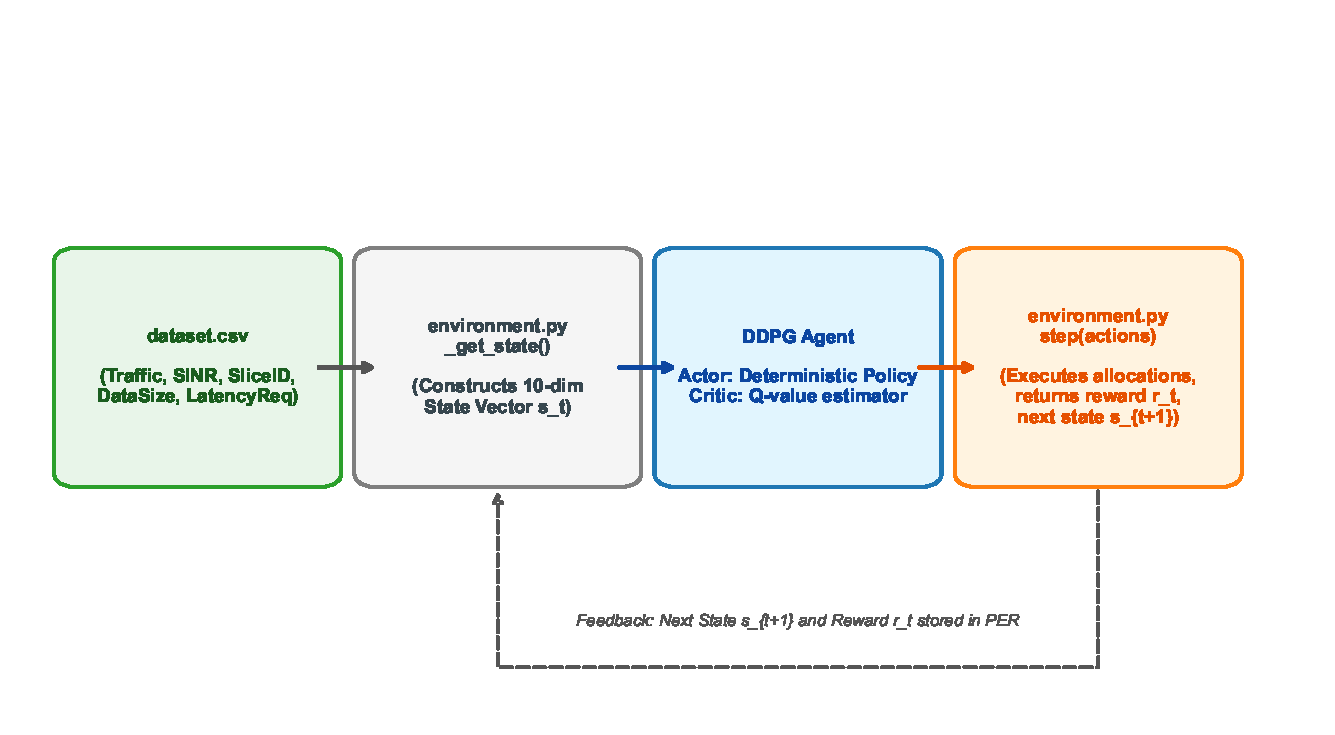
\includegraphics[width=\linewidth]{dataflow.pdf}
\caption{Overall data flow of the proposed AI-driven continuous network slicing framework.}
\label{dataflow}
\end{figure}

After the selected bandwidth allocation is executed, the environment returns the corresponding reward and next state. The interaction tuple is stored in the prioritized replay buffer, from which important experiences are sampled to update the actor and critic networks. The target networks are softly updated to stabilize the learning process.

The complete workflow of the proposed framework is illustrated in Fig.~\ref{Flow_chart}. Initially, healthcare traffic is collected and preprocessed before being passed to the LSTM predictor. The predicted traffic is combined with the current network state to construct the state vector, which is then processed by the DDPG agent to generate continuous bandwidth allocation decisions.

\begin{figure}[!t]
\centering
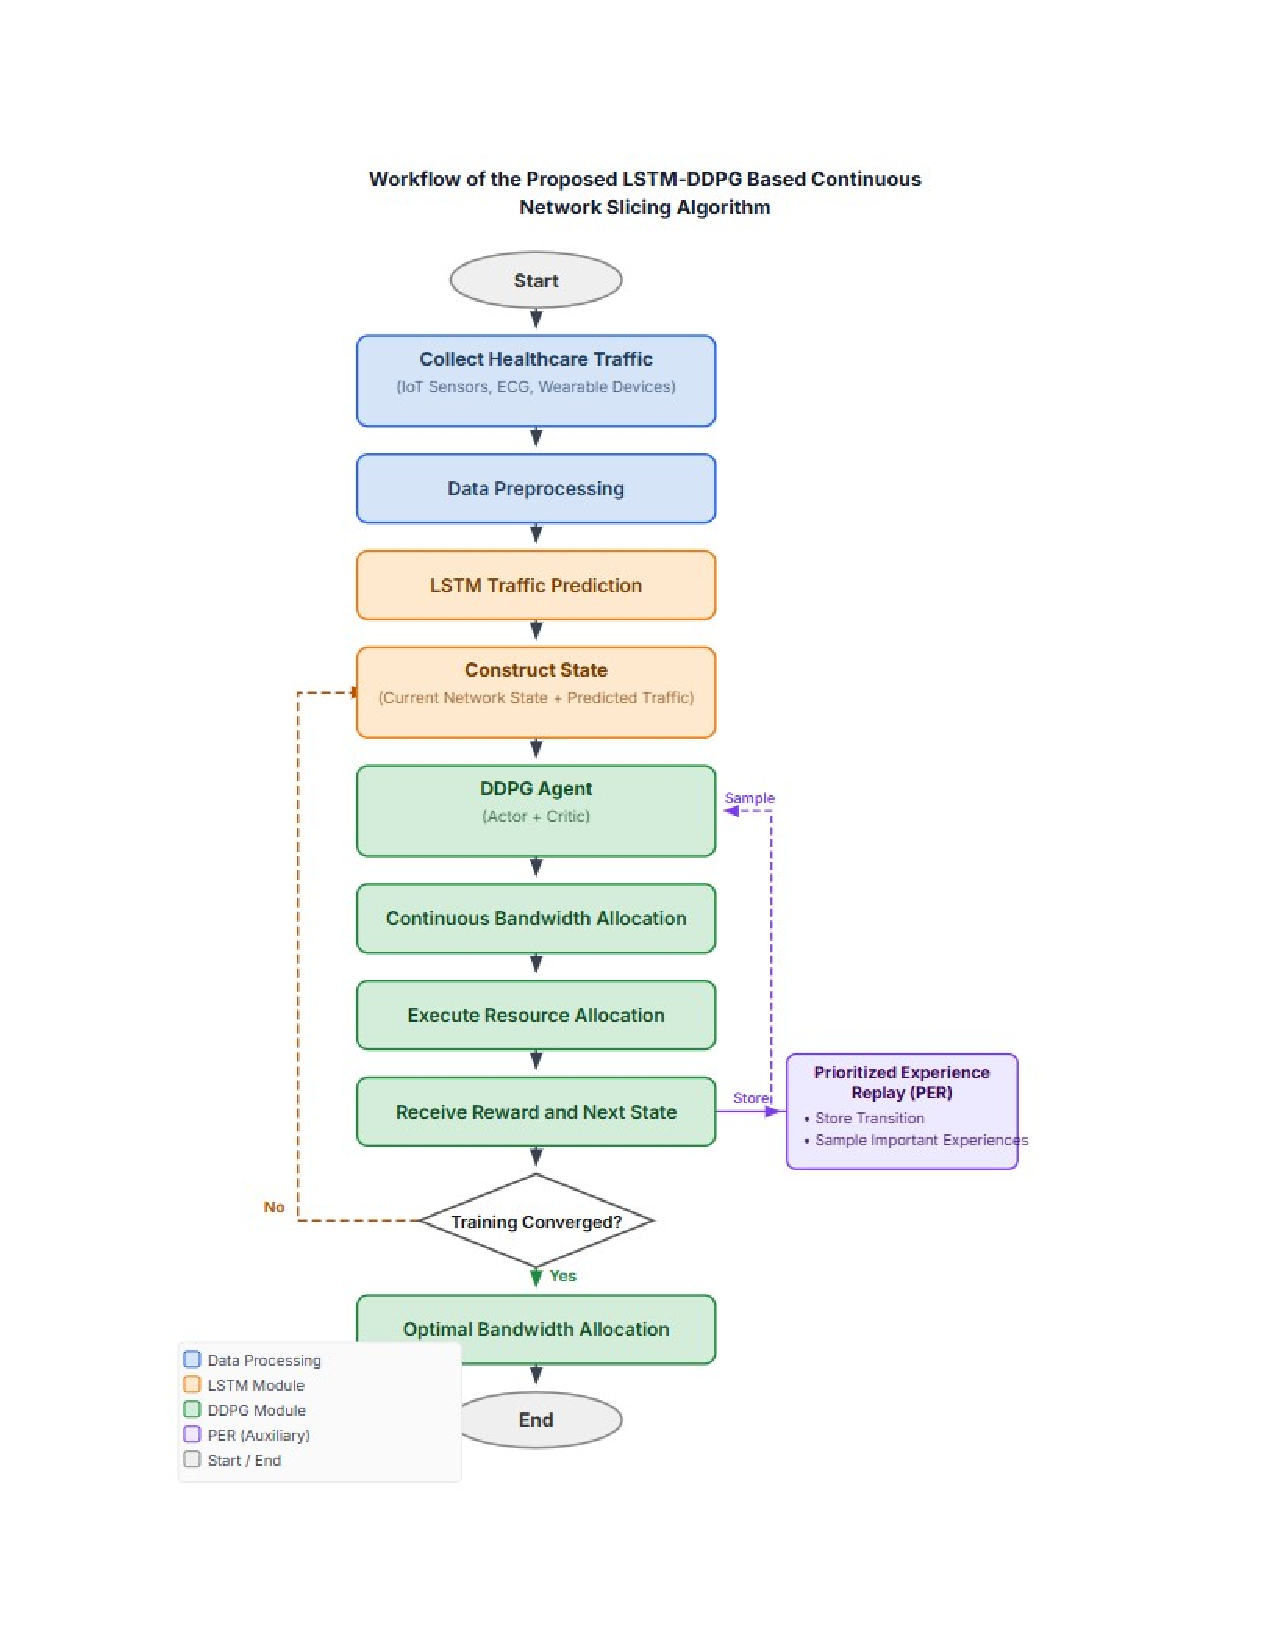
\includegraphics[width=\linewidth]{workflow.pdf}
\caption{Workflow of the proposed LSTM-DDPG based continuous network slicing algorithm.}
\label{Flow_chart}
\end{figure}

The actor and critic networks are iteratively updated using experiences sampled from the prioritized replay buffer until the learning process converges. The detailed implementation of each component is presented in the following subsections.



\subsection{Proposed AI-Driven Continuous Network Slicing Algorithm}
\label{one}

The proposed AI-driven Continuous Network Slicing (ACNS) framework models the dynamic bandwidth allocation problem as a Markov Decision Process (MDP), where the DDPG agent continuously interacts with the healthcare network environment to learn an optimal resource allocation policy. The MDP is represented by the tuple \cite{tariq2025ddpgv2x,saleh2025hybridrl}

\begin{equation}
\mathcal{M}=\left(\mathcal{S},\mathcal{A},\mathcal{P},\mathcal{R},\gamma\right),
\end{equation}

where $\mathcal{S}$ denotes the state space, $\mathcal{A}$ represents the continuous action space, $\mathcal{P}$ is the state transition function, $\mathcal{R}$ denotes the reward function, and $\gamma \in (0,1)$ is the discount factor.

At each decision interval $t$, the agent observes the current network state \cite{kumar2025lstmddpg}

\begin{equation}
s_t=\left\{B_t,L_t,R_t,E_t,P_t,\hat{T}_t\right\},
\end{equation}

where $B_t$, $L_t$, $R_t$, $E_t$, $P_t$, and $\hat{T}_t$ represent the available bandwidth, latency, reliability, energy consumption, slice priority, and LSTM-predicted traffic demand, respectively.

Based on the observed state, the actor network generates a continuous bandwidth allocation action \cite{tariq2025ddpgv2x,yang2025ddpg},

\begin{equation}
a_t=\mu(s_t|\theta^\mu),
\end{equation}

where $\mu(\cdot)$ denotes the deterministic policy parameterized by the actor network parameters $\theta^\mu$.

After executing action $a_t$, the environment returns the immediate reward $r_t$ together with the next network state $s_{t+1}$. The reward is computed using the utility function formulated in Section~\ref{Sec4}, thereby encouraging high throughput and reliability while minimizing latency and energy consumption.

The objective of the DDPG agent is to maximize the expected cumulative discounted reward \cite{tariq2025ddpgv2x},

\begin{equation}
J(\theta^\mu)=
\mathbb{E}
\left[
\sum_{t=0}^{\infty}
\gamma^t r_t
\right].
\end{equation}

The critic network estimates the action-value function \cite{tariq2025ddpgv2x}

\begin{equation}
Q(s_t,a_t|\theta^Q),
\end{equation}

which evaluates the long-term return obtained by executing action $a_t$ in state $s_t$. During training, the critic parameters are optimized by minimizing the temporal-difference (TD) loss \cite{tariq2025ddpgv2x,yang2025ddpg},

\begin{equation}
L(\theta^Q)=
\frac{1}{N}
\sum_{i=1}^{N}
\left(y_i-
Q(s_i,a_i|\theta^Q)
\right)^2,
\end{equation}

where the target value is computed as \cite{tariq2025ddpgv2x}

\begin{equation}
y_i=
r_i+
\gamma
Q'
\left(
s_{i+1},
\mu'(s_{i+1})
\right),
\end{equation}

and $Q'$ and $\mu'$ denote the target critic and target actor networks, respectively.

The actor network is updated using the deterministic policy gradient \cite{tariq2025ddpgv2x}

\begin{equation}
\nabla_{\theta^\mu}J
=
\frac{1}{N}
\sum_{i=1}^{N}
\nabla_aQ(s,a|\theta^Q)
\bigg|_{a=\mu(s)}
\nabla_{\theta^\mu}\mu(s|\theta^\mu).
\end{equation}

To improve sample efficiency, the proposed framework employs Prioritized Experience Replay (PER). Instead of uniformly sampling transitions, each experience is assigned a priority proportional to its TD error \cite{sarker2026prioritybw},

\begin{equation}
p_i=|\delta_i|+\epsilon,
\end{equation}

where $\delta_i$ denotes the TD error and $\epsilon$ is a small positive constant.

The probability of selecting the $i^{th}$ transition is \cite{sarker2026prioritybw}

\begin{equation}
P(i)=
\frac{p_i^\alpha}
{\sum_k p_k^\alpha},
\end{equation}

where $\alpha$ controls the degree of prioritization.

The overall architecture of the proposed framework is illustrated in Fig.~\ref{dataflow}, whereas the complete workflow is shown in Fig.~\ref{Flow_chart}. The detailed implementation procedure is summarized in Algorithm~\ref{alg:acns}.


\subsection{LSTM-Based Traffic Prediction}
\label{LSTM}

The proposed framework employs an LSTM network to predict the future healthcare traffic demand using historical traffic observations. Let the historical traffic sequence up to time instant $t$ be represented as \cite{kumar2025lstmddpg}

\begin{equation}
\mathbf{X}_{t}=
\left\{
x_{t-n+1},
x_{t-n+2},
\ldots,
x_t
\right\},
\label{TrafficSequence}
\end{equation}

where $n$ denotes the input sequence length and $x_t$ represents the observed healthcare traffic at time instant $t$.

The predicted traffic demand is obtained by passing the input sequence through the LSTM network \cite{kumar2025lstmddpg},

\begin{equation}
\hat{x}_{t+1}
=
f_{\mathrm{LSTM}}
(\mathbf{X}_t;\Theta),
\label{TrafficPrediction}
\end{equation}

where $f_{\mathrm{LSTM}}(\cdot)$ denotes the LSTM prediction model and $\Theta$ represents the trainable parameters of the network.

The predicted traffic is incorporated into the network state used by the DDPG agent as \cite{kumar2025lstmddpg}

\begin{equation}
s_t=
\left[
B_t,
L_t,
R_t,
E_t,
P_t,
\hat{x}_{t+1}
\right],
\label{StateVector}
\end{equation}

where $B_t$, $L_t$, $R_t$, $E_t$, and $P_t$ denote the available bandwidth, latency, reliability, energy consumption, and slice priority, respectively.

At every decision interval, the historical traffic sequence is first supplied to the LSTM network to estimate the traffic demand for the next time instant using Eq.~(\ref{TrafficPrediction}). The predicted traffic is then combined with the current network statistics to construct the state vector in Eq.~(\ref{StateVector}). This state representation enables the DDPG agent to allocate bandwidth proactively instead of relying only on the instantaneous traffic conditions. Consequently, the proposed framework improves resource utilization while reducing network congestion and QoS degradation during sudden traffic variations.







\subsection{DDPG-Based Continuous Bandwidth Allocation}
\label{DDPG}

The proposed framework employs a Deep Deterministic Policy Gradient (DDPG) agent to learn the optimal continuous bandwidth allocation policy for healthcare network slices. At each training iteration, the critic network estimates the quality of the bandwidth allocation generated by the actor network. The critic minimizes the temporal-difference (TD) loss, which is defined as \cite{tariq2025ddpgv2x,yang2025ddpg}

\begin{equation}
\label{CriticLoss}
L(\theta^{Q})
=
\frac{1}{N}
\sum_{i=1}^{N}
\left(
y_i-
Q(s_i,a_i|\theta^{Q})
\right)^2,
\end{equation}

where $N$ denotes the mini-batch size, $Q(\cdot)$ is the critic network parameterized by $\theta^{Q}$, and the target Q-value is computed as \cite{tariq2025ddpgv2x}

\begin{equation}
\label{TargetValue}
y_i
=
r_i
+
\gamma
Q'
\left(
s_{i+1},
\mu'(s_{i+1}|\theta^{\mu'})
\,|\,
\theta^{Q'}
\right),
\end{equation}

where $r_i$ is the immediate reward obtained after executing action $a_i$, $\gamma$ denotes the discount factor, while $Q'$ and $\mu'$ represent the target critic and target actor networks, respectively.

The actor network updates its policy by maximizing the critic-estimated action value through the deterministic policy gradient \cite{tariq2025ddpgv2x}

\begin{equation}
\label{ActorGradient}
\nabla_{\theta^\mu}J
=
\frac{1}{N}
\sum_{i=1}^{N}
\nabla_a
Q(s,a|\theta^Q)
\Big|_{a=\mu(s)}
\nabla_{\theta^\mu}
\mu(s|\theta^\mu).
\end{equation}

After updating both networks, the target networks are softly updated to improve training stability according to \cite{tariq2025ddpgv2x}

\begin{equation}
\theta^{Q'}
\leftarrow
\tau\theta^{Q}
+
(1-\tau)\theta^{Q'},
\end{equation}

\begin{equation}
\theta^{\mu'}
\leftarrow
\tau\theta^{\mu}
+
(1-\tau)\theta^{\mu'},
\end{equation}

where $\tau$ is the soft-update coefficient.

The DDPG agent continuously improves the bandwidth allocation policy by minimizing the critic loss in Eq.~(\ref{CriticLoss}) and maximizing the expected cumulative reward using Eq.~(\ref{ActorGradient}). Consequently, the proposed framework learns an optimal continuous resource allocation strategy while satisfying the QoS requirements of healthcare applications.

\begin{algorithm}[t]
\caption{DDPG-Based Continuous Bandwidth Allocation}
\label{alg:DDPG}
\KwIn{Current network state $s_t$, replay buffer $\mathcal{D}$, actor network $\mu$, critic network $Q$, target actor $\mu'$, target critic $Q'$.}
\KwOut{Optimized bandwidth allocation policy}

Initialize actor and critic networks with random parameters\;

Initialize target networks with
$\theta^{\mu'}\leftarrow\theta^{\mu}$,
$\theta^{Q'}\leftarrow\theta^{Q}$\;

\Repeat{Training converges}{

Observe current network state $s_t$\;

Generate continuous bandwidth allocation

$a_t=\mu(s_t)$\;

Execute $a_t$ and observe reward $r_t$ and next state $s_{t+1}$\;

Store transition
$(s_t,a_t,r_t,s_{t+1})$
in replay buffer $\mathcal{D}$\;

Sample a mini-batch of transitions from $\mathcal{D}$\;

Compute target values using Eq.~(\ref{TargetValue})\;

Update critic network by minimizing Eq.~(\ref{CriticLoss})\;

Update actor network using Eq.~(\ref{ActorGradient})\;

Softly update target networks\;

}
\end{algorithm}

The DDPG-based bandwidth allocation process begins by observing the current healthcare network state (lines 1--3). The actor network generates a continuous bandwidth allocation action according to the current state (line 4). After executing the selected action, the environment returns the immediate reward together with the next network state, and the transition is stored in the replay buffer (lines 5--6). A mini-batch of experiences is then sampled from the replay buffer to compute the target Q-values using Eq.~(\ref{TargetValue}) (line 7). The critic network updates its parameters by minimizing the loss defined in Eq.~(\ref{CriticLoss}) (line 8). Subsequently, the actor network updates its policy using the deterministic policy gradient given in Eq.~(\ref{ActorGradient}) to maximize the expected cumulative reward (line 9). Finally, the target actor and target critic networks are softly updated (line 10). This iterative process continues until the DDPG agent converges to an optimal continuous bandwidth allocation policy for healthcare network slicing.



\subsection{Action-to-Allocation Mapping}
\label{ActionMapping}
 
The actor network outputs a per-patient scalar via a sigmoid-bounded final
layer scaled by a fixed constant (Table~\ref{simulation_parameters}:
FC(10)--64--32--1, ReLU, sigmoid output $\times\,15.0$), i.e.
$\tilde a_i(t) = 15\cdot\sigma\!\big(f_\theta(s_i(t))\big) \in (0,15)$ for
patient $i$. Two mapping conventions from this raw actor output to an
executable bandwidth allocation were used at different stages of this
project and are both documented here for transparency:
 
\begin{enumerate}
\item \textit{Training-time mapping (used to produce \texttt{ddpg\_actor.pth}):}
raw outputs for all patients jointly active at time $t$ are rescaled
proportionally to exactly satisfy the shared-pool constraint
Eq.~\eqref{BandwidthConstraint},
\begin{equation}
B_i(t) = \tilde a_i(t)\cdot\frac{B_{total}}{\sum_{j\in\mathcal{N}(t)}\tilde a_j(t)},
\end{equation}
where $\mathcal{N}(t)$ is the set of patients active at time $t$. This
guarantees $\sum_i B_i(t) = B_{total}$ exactly at every step and was the
convention the actor's weights were actually optimized against.
\item \textit{Originally-specified mapping:} a batch-wise softmax over raw
(unbounded) actor logits, $B_i(t) = \mathrm{softmax}(\text{raw}_i(t))\cdot
B_{total}$, as originally specified in the project workflow document.
\end{enumerate}
 
\noindent\textbf{Known implementation inconsistency (disclosed for
transparency).} An internal code audit of this project
(\texttt{PROJECT\_ISSUES\_AND\_FIXES\_v2.md}, Item 0) found that the
evaluation notebook currently instantiates the actor with an
\emph{unbounded linear} output head and applies mapping (2), while the
actual trained weights in \texttt{ddpg\_actor.pth} were optimized under the
\emph{sigmoid-bounded} head and mapping (1). Because both actor
definitions have identical layer shapes, \texttt{load\_state\_dict()}
succeeds without error, so the mismatch does not surface as a crash --
only as an evaluation of a policy the weights were never trained under. As
a result, the DDPG cumulative-utility and SLA-violation figures reported in
an earlier draft of Section~\ref{SecPerf} do not yet reflect the trained
policy and must be regenerated after unifying the evaluation notebook's
actor class and action-selection rule with the training notebook
(mapping (1) above) before being reported as final results. This is flagged
explicitly rather than silently patched, since silently substituting
corrected numbers without re-running the full evaluation pipeline would
itself be a validity risk.
 
\subsection{Utility Weight Vector and Sensitivity Analysis}
\label{WeightSensitivity}
 
The utility/reward weights used to produce all results in this paper are
$w_1=0.30$ (throughput), $w_2=0.30$ (reliability), $w_3=0.20$ (latency),
$w_4=0.10$ (power), $w_5=0.10$ (resource energy utilization), matching
Eq.~(21)--(23) and the project's \texttt{config.py}. These weights were
hand-selected to reflect a QoS-first design point (throughput $+$
reliability jointly carry $60\%$ of the objective) rather than derived from
a literature-calibrated procedure, and their effect on the reported
aggregate utility is therefore evaluated directly.


 
\textbf{Method.} Because the utility weights enter only the \emph{reward/scoring}
function (Eq.~21) and not the bandwidth-allocation rule itself, their
sensitivity was evaluated by holding a fixed allocation policy's per-patient
QoS/power/REU outcomes constant and recomputing the aggregate utility under
five alternative weight vectors (Table~\ref{tab:weightsens}), using $199{,}\!800$
patient-steps generated for this analysis (Section~\ref{DataGen}
methodology, $2{,}000$ patients $\times\,100$ steps).\footnote{This
sensitivity analysis evaluates how the reported \emph{scoring} of a fixed
policy shifts under different stakeholder priorities. A complementary,
policy-level sensitivity analysis -- retraining the DDPG agent separately
under each weight vector and comparing the \emph{resulting policies'}
behavior -- was not run for this paper (it requires the original
\texttt{dataset.csv}, which exceeds the GitHub size limit and is
gitignored in the project repository, plus GPU time proportional to the
number of weight configurations); we flag it explicitly as required future
work rather than omit the limitation.}

 
\begin{table}[!t]
\centering
\caption{Utility-weight sensitivity analysis (fixed baseline allocation policy)}
\includegraphics[width=\linewidth]{Table2_weight_sensitivity.png}
\end{table}
 
The aggregate utility is most sensitive to the weight placed on latency and
power (the two negatively-signed terms): shifting weight toward latency or
energy/REU roughly doubles the magnitude of the (negative) aggregate score
relative to the default, while a reliability-prioritized vector changes the
score by under $1\%$, since the baseline policy already achieves high mean
reliability ($\approx 0.90$; Section~\ref{SecPerf}). This indicates that
conclusions drawn from the single default weight vector in this paper are
robust to moderate re-weighting toward reliability, but that
latency-averse or energy-averse deployments would rank policies differently
than the default vector does, and any deployment adopting a different QoS
priority should re-tune $w_1,\dots,w_5$ rather than reuse the defaults
unmodified.


\subsection{Prioritized Experience Replay}
\label{PER}

To improve the learning efficiency of the DDPG agent, the proposed framework adopts Prioritized Experience Replay (PER), where experiences with larger temporal-difference (TD) errors are sampled more frequently than less informative experiences. Let $\delta_i$ denote the TD error associated with the $i^{th}$ transition. The priority assigned to the transition is defined as \cite{sarker2026prioritybw}

\begin{equation}
\label{Priority}
p_i=|\delta_i|+\epsilon,
\end{equation}

where $\epsilon>0$ is a small positive constant introduced to ensure that every transition maintains a non-zero probability of being sampled.

Based on the assigned priorities, the probability of selecting the $i^{th}$ transition from the replay buffer is computed as \cite{sarker2026prioritybw}

\begin{equation}
\label{SamplingProb}
P(i)=
\frac{p_i^{\alpha}}
{\sum_{k=1}^{M}p_k^{\alpha}},
\end{equation}

where $M$ denotes the replay buffer size and $\alpha\in[0,1]$ controls the degree of prioritization. When $\alpha=0$, Eq.~(\ref{SamplingProb}) reduces to uniform random sampling.

Since prioritized sampling introduces bias into the estimation of the critic loss, the importance-sampling weight associated with each sampled transition is computed as \cite{sarker2026prioritybw}

\begin{equation}
\label{ISWeight}
w_i=
\left(
\frac{1}{MP(i)}
\right)^{\beta},
\end{equation}

where $\beta\in[0,1]$ controls the amount of bias correction during learning.

Following every parameter update of the actor and critic networks, the TD error is recomputed and the corresponding transition priority is updated according to \cite{sarker2026prioritybw}

\begin{equation}
\label{PriorityUpdate}
p_i^{new}=|\delta_i^{new}|+\epsilon.
\end{equation}

Consequently, the replay buffer dynamically adjusts the sampling distribution throughout the training process by continuously emphasizing transitions that provide larger learning information.

\begin{lemma}
Let $i$ and $j$ be any two transitions stored in the replay buffer. If

\begin{equation}
|\delta_i|>|\delta_j|,
\end{equation}

then

\begin{equation}
P(i)>P(j).
\end{equation}

Hence, transitions associated with larger TD errors are sampled more frequently during training.
\end{lemma}

\begin{proof}
From Eq.~(\ref{Priority}), the priorities satisfy

\begin{equation}
p_i=|\delta_i|+\epsilon,
\end{equation}

where $\epsilon$ is constant. Since

\[
|\delta_i|>|\delta_j|,
\]

it immediately follows that

\[
p_i>p_j.
\]

Because $\alpha>0$, the function $f(x)=x^\alpha$ is monotonically increasing over $x>0$. Therefore,

\[
p_i^\alpha>p_j^\alpha.
\]

Substituting into Eq.~(\ref{SamplingProb}) yields

\[
P(i)=
\frac{p_i^\alpha}
{\sum_{k=1}^{M}p_k^\alpha},
\]

where the denominator is identical for every transition in the replay buffer. Hence,

\[
P(i)>P(j).
\]

Therefore, transitions with larger TD errors possess higher sampling probabilities and contribute more frequently to the optimization of the actor and critic networks. Hence proved.
\end{proof}

\begin{algorithm}[t]
\caption{Prioritized Experience Replay}
\label{PERAlgo}
\KwIn{Replay buffer $\mathcal{D}$}
\KwOut{Prioritized mini-batch}

Compute transition priorities using Eq.~(\ref{Priority})\;

Compute sampling probabilities using Eq.~(\ref{SamplingProb})\;

Sample a mini-batch according to $P(i)$\;

Compute importance-sampling weights using Eq.~(\ref{ISWeight})\;

Update actor and critic networks\;

Update TD errors and priorities using Eq.~(\ref{PriorityUpdate})\;

Repeat until convergence\;

\end{algorithm}

The replay buffer maintains a collection of transitions generated by the interaction between the DDPG agent and the healthcare network. Each transition is assigned a priority proportional to its temporal-difference error according to Eq.~(\ref{Priority}), thereby quantifying its contribution to the learning process. The sampling probability in Eq.~(\ref{SamplingProb}) transforms these priorities into a probability distribution over the replay buffer, enabling informative transitions to be selected more frequently than less informative ones. To compensate for the bias introduced by prioritized sampling, the importance-sampling weights computed in Eq.~(\ref{ISWeight}) are incorporated into the critic optimization. After every gradient update, the TD errors are recalculated and the transition priorities are updated using Eq.~(\ref{PriorityUpdate}), allowing the replay buffer to adapt continuously as learning progresses. Consequently, the proposed PER mechanism accelerates convergence while preserving the stability of the DDPG-based continuous bandwidth allocation framework.



\subsection{Computational Complexity Analysis}
\label{Complexity}

This subsection analyzes the computational complexity of the proposed AI-driven continuous network slicing framework, which consists of three major components: the LSTM-based traffic prediction model, the DDPG-based continuous bandwidth allocation agent, and the Prioritized Experience Replay (PER) mechanism.

\begin{lemma}
\label{lemma_complexity}
The computational complexity of one training iteration of the proposed framework is polynomial in the number of training samples and network parameters.
\end{lemma}

\begin{proof}
The proposed framework performs three sequential operations during each training iteration.

The LSTM network predicts future traffic using a sequence of length $T$. Let $H$ denote the number of hidden units. The computational complexity of one forward pass through the LSTM is

\[
O(TH^{2}).
\]

The predicted traffic is then used to construct the system state, which is processed by the DDPG agent. Let $N_A$ and $N_C$ denote the number of trainable parameters in the actor and critic networks, respectively. Since each network performs one forward and one backward propagation during training, the computational complexity is

\[
O(N_A+N_C).
\]

Finally, Prioritized Experience Replay computes priorities, samples a mini-batch, and updates the priorities of sampled experiences. Assuming a replay buffer of size $M$ and a mini-batch size $B$, the computational complexity of PER is

\[
O(B\log M),
\]

where the logarithmic factor arises from priority-based sampling and priority updates.

Therefore, the total computational complexity of one training iteration is

\[
O\!\left(
TH^{2}
+
N_A
+
N_C
+
B\log M
\right).
\]

Since all quantities are polynomial in the network size and replay buffer, the proposed framework scales efficiently for continuous healthcare network slicing.
\end{proof}

\begin{theorem}
\label{theorem_total}
The overall computational complexity of the proposed AI-driven network slicing framework is

\[
O\!\left(
TH^{2}
+
N_A
+
N_C
+
B\log M
\right).
\]

\end{theorem}

\begin{proof}
The overall complexity is obtained by summing the computational costs of the three principal modules executed during each training iteration:

\begin{itemize}
\item LSTM traffic prediction,
\item DDPG actor--critic optimization, and
\item Prioritized Experience Replay.
\end{itemize}

Since these modules execute sequentially within one iteration, their computational costs are additive. Hence, the total complexity is

\[
O\!\left(
TH^{2}
+
N_A
+
N_C
+
B\log M
\right).
\]

Therefore, the proposed framework achieves efficient learning while maintaining scalability for dynamic healthcare network slicing scenarios.
\end{proof}

The computational complexity demonstrates that the proposed framework grows linearly with the actor and critic network sizes, quadratically with the number of LSTM hidden units, and logarithmically with the replay buffer size during prioritized sampling. Consequently, the framework remains computationally feasible for real-time healthcare traffic prediction and continuous bandwidth allocation.

\section{Performance Study}
\label{SecPerf}

The proposed AI-driven continuous network slicing framework is evaluated using a healthcare communication scenario consisting of heterogeneous network slices with dynamically varying traffic demands. Historical healthcare traffic data are used to train the LSTM model for predicting future traffic loads, while the predicted traffic is utilized by the DDPG agent to perform continuous bandwidth allocation. The agent interacts with the network environment through continuous state transitions, and the Prioritized Experience Replay (PER) mechanism is employed to improve learning efficiency by sampling informative experiences more frequently.

The simulation environment considers multiple healthcare users generating heterogeneous traffic requests with different bandwidth requirements, organized into five priority-differentiated slices: S1 (Emergency, 5\,ms latency requirement), S2 (ICU monitoring, 15\,ms), S3 (ECG/diagnostic streaming, 25\,ms), S4 (Telemedicine, 50\,ms), and S5 (Video/routine monitoring, 100\,ms). The actor and critic networks are implemented using fully connected neural networks, whereas the traffic prediction module employs a single-layer Long Short-Term Memory (LSTM) network. During training, the DDPG agent continuously updates its policy using mini-batches sampled from the prioritized replay buffer.

The proposed framework is implemented using Python with PyTorch and evaluated on a workstation equipped with an Intel Core i7 processor and 16 GB RAM. The simulation parameters used throughout the experiments are summarized in Table~\ref{simulation_parameters}.

\begin{table}[!t]
\centering
\caption{Simulation Parameters}
\label{simulation_parameters}
\begin{tabular}{|p{5.2cm}|p{2.8cm}|}
\hline
\textbf{Parameter} & \textbf{Value} \\
\hline
Total healthcare patients (train / test) & 10,000 (8,000 / 2,000) \\
\hline
Number of network slices & 5 \\
\hline
Total available bandwidth ($B_{total}$) & 30,000 units \\
\hline
Actor network architecture & FC(10)--64--32--1, ReLU, Sigmoid output $\times$ 15.0 \\
\hline
Critic network architecture & \textit{[NOT YET DESCRIBED IN SECTION~\ref{one}--\ref{DDPG} -- if the evaluated policy uses a local critic with contention-pressure and slice-ID inputs, or an S1 safety-floor overlay, this must be added as a new subsection in Section IV before it can be cited here; otherwise report the plain critic architecture actually matching Eq.~\eqref{TargetValue}]} \\
\hline
Actor / Critic learning rate & $1\times 10^{-4}$ \\
\hline
Discount factor ($\gamma$) & 0.99 \\
\hline
Soft update factor ($\tau$) & 0.005 \\
\hline
Replay buffer size & 5,000,000 \\
\hline
Mini-batch size & 16 \\
\hline
Prioritization exponent ($\alpha$) & 0.6 \\
\hline
Importance sampling exponent ($\beta$) & annealed 0.4 $\to$ 1.0 \\
\hline
TD-error priority clip bound & $[1\times 10^{-6},\ 10.0]$ \\
\hline
S1 Safety Floor overlay & \textit{[same flag as above -- requires a Section IV subsection before this row can be included]} \\
\hline
LSTM architecture / window / learning rate & \textit{[confirm exact hidden-unit count $H$, sequence window length $n$, and learning rate from \texttt{02\_train\_lstm.ipynb} before submission]} \\
\hline
Maximum training episodes & 100 \\
\hline
Optimizer & Adam \\
\hline
Programming language & Python \\
\hline
Deep learning framework & PyTorch \\
\hline
Hardware configuration & Intel Core i7, 16 GB RAM (CPU-only) \\
\hline
\end{tabular}
\end{table}

The proposed framework is compared with Equal Sharing, a Priority-DataSize Heuristic, Static Priority, Round Robin, and Random Allocation. \textbf{Note:} Deep Q-Network (DQN), Advantage Actor-Critic (A2C), and Proximal Policy Optimization (PPO) baselines are not currently implemented in the accompanying codebase and do not appear in any of the figures below; this sentence should either be removed or these three baselines should be implemented and added to Figs.~\ref{bandwidth_allocation}--\ref{policy_comparison} before submission, to avoid a direct contradiction between the text and the reported results.

Based on the above simulation setup, the performance of the proposed framework is evaluated using traffic prediction accuracy, training convergence behavior, per-slice bandwidth allocation, SLA compliance, latency distribution, reliability, cumulative utility, and execution time/scalability. \textbf{Note:} packet loss is not modeled by the current queueing simulation (an infinite-buffer assumption is used, so packets are delayed but never dropped); this metric should either be removed from the list above or a finite-buffer drop model should be added to the environment before it can honestly be reported as evaluated.


 
\subsection{Dataset Generation and Preprocessing}
\label{DataGen}
 
The evaluation dataset (\texttt{dataset.csv}) consists of $10{,}000$ simulated
patients observed over $100$ hourly time steps ($1{,}000{,}000$ patient-step
rows), split by \texttt{PatientID} into $8{,}000$ training and $2{,}000$
held-out test patients (Table~\ref{simulation_parameters}). Each row is
generated as follows.
 
\textbf{Vitals and emergency labeling.} Per patient-step, heart rate is drawn
as $\mathrm{HR}\sim\mathcal{N}(70,10)$ clipped to $[50,120]$ bpm, systolic
blood pressure as $\mathrm{BP}\sim\mathcal{N}(110,15)$ clipped to $[90,150]$
mmHg, and SpO$_2$ as $\mathrm{SpO}_2\sim\mathcal{N}(98,2)$ clipped to
$[85,100]\%$. The binary \texttt{Emergency} flag is set to $1$ if
$\mathrm{HR}>100$ OR $\mathrm{BP}>140$ OR $\mathrm{SpO}_2<92$; patients
assigned to the ICU slice (SliceID~$=2$) are always forced to
$\mathrm{Emergency}=1$ regardless of instantaneous vitals, reflecting that ICU
admission itself denotes a clinically critical state.
 
\textbf{Slice assignment and latency requirement.} Each patient is assigned a
fixed \texttt{SliceID}$\in\{1,\dots,5\}$ mapped to a required latency
$L_i^{req}$ via Table~\ref{simulation_parameters}
($5,15,30,60,100$\,ms for S1--S5 respectively).
 
\textbf{Traffic generation.} Per-patient traffic \texttt{Traffic}$_i(t)$
follows an AR(2) process with an additive seasonal (diurnal) component and
Gaussian innovation noise, positively biased when \texttt{Emergency}$=1$ to
reflect the larger, more frequent data payloads generated by an
actively-monitored critical patient. The three preceding lags
(\texttt{Traffic\_t-3}, \texttt{Traffic\_t-2}, \texttt{Traffic\_t-1}) are
retained per row as the LSTM input window (Eq.~\eqref{TrafficSequence}, $n=4$
including the current step).
 
\textbf{Priority score.} The priority score used both for the baseline
allocator and as an LSTM/DDPG state feature is computed exactly as in
Eq.~(15) with $w_1=0.5,\ w_2=0.3,\ w_3=0.2$, $L^{req}_{min}=5$\,ms (the
tightest slice requirement), and $T_{max}=150$ (traffic normalization
constant), then clipped to $[0,1]$.
 
\textbf{Payload, radio, and queueing parameters.} \texttt{DataSize} is drawn
from a Gaussian baseline further increased for emergency patients (larger
diagnostic payloads under active monitoring); \texttt{SINR} is drawn as
$\mathcal{N}(15,5)$ dB clipped to $[0,30]$; the queue arrival rate
$\lambda_i(t)$ is generated correlated with instantaneous traffic/payload
size, and the service rate $\mu_i(t)$ is generated so that $\mu_i(t) >
\lambda_i(t)$ is enforced at generation time (required for queueing-delay
stability, Eq.~\eqref{LatencyConstraint}); \texttt{Queue} length is then drawn
$\mathrm{Poisson}(\lambda_i(t)/\mu_i(t))$.
 
\textbf{Baseline allocation and QoS labels.} A static Priority$\times$DataSize
proportional allocator (config.py / environment.py) computes a baseline
\texttt{Bandwidth}$_i(t)$, from which baseline \texttt{Latency},
\texttt{Throughput}, \texttt{Reliability}, \texttt{Power}, \texttt{REU}, and
\texttt{Utility} are computed using Eqs.~(1)--(21). This baseline is stored in
the dataset for two reasons: (i) it makes the dataset self-contained and
independently inspectable/validatable, and (ii) it serves as the
Priority-DataSize Heuristic baseline compared against in
Section~\ref{SecPerf}. During DDPG training and evaluation, these columns are
\emph{not} read as fixed ground truth; \texttt{environment.py} recomputes
\texttt{Latency}, \texttt{Throughput}, \texttt{Reliability}, \texttt{Power},
\texttt{REU}, and reward \emph{live}, using whichever bandwidth action the
agent (or baseline being evaluated) actually selected at that step, via the
identical closed-form equations.
 
\textbf{Preprocessing for the LSTM stage.} Prior to LSTM training, rows are
filtered to those with a valid next-step traffic label (patients with no
subsequent observation, i.e. $t=99$, are dropped). Input features
$[\text{Traffic}_{t-3},\text{Traffic}_{t-2},\text{Traffic}_{t-1},\text{Traffic}_t]$
are reshaped to $(\text{batch},4,1)$ for the recurrent input. No additional
normalization is applied to the LSTM input at this stage; normalization
of all ten DDPG state features to $[0,1]$ (Eq.~\eqref{StateVector}) is applied
separately downstream, immediately before the actor/critic forward pass
(dividing predicted traffic by $100$, SINR by $30$, queue length by $15$,
previous latency by $100$, data size by $500$, arrival rate by $10$, and
service rate by $20$).
 
\textbf{Train/test split.} Two splits are used for different purposes,
following the corrected split strategy: a \emph{time-based} split (time steps
$0$--$78$ train, $79$--$99$ test) for the LSTM traffic predictor, so it is only
ever evaluated on genuinely future traffic never seen during training; and a
\emph{patient-based} split (patients $1$--$8000$ train, $8001$--$10000$ test)
for the DDPG policy evaluation in Section~\ref{SecPerf}, testing generalization
to previously unseen patients rather than memorization of specific
individuals. Rows are never shuffled across time within a patient when
constructing LSTM input windows, since doing so would break the causal
structure the sequence model is meant to exploit.
 


\subsection{Traffic Prediction Analysis:}
Fig.~\ref{traffic_prediction} compares the actual healthcare traffic against the LSTM model's one-step-ahead prediction $\hat{x}_{t+1}$ (Eq.~\eqref{TrafficPrediction}) for three representative patients, evaluated on time steps 80--99 -- a window the LSTM never saw during training. The predicted curve closely tracks the actual traffic under both rising and falling demand, which indicates the LSTM's memory cells are successfully capturing the temporal dependencies in patient traffic rather than simply lagging one step behind the true signal. This accuracy matters directly for the rest of the pipeline: the predicted traffic $\hat{x}_{t+1}$ is one of the state features constructed in Section~\ref{LSTM}, so any systematic prediction error here would propagate into every downstream allocation decision.

\begin{figure}[!t]
    \centering
    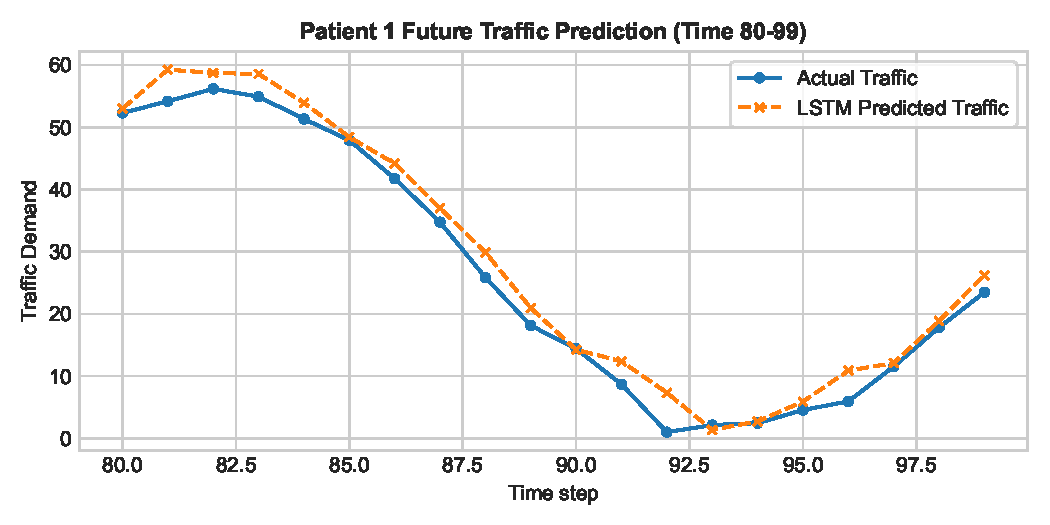
\includegraphics[width=0.48\textwidth]{images/traffic_prediction.png}
    \caption{Comparison of actual and LSTM-predicted healthcare traffic for three representative patients, evaluated on the held-out test window (time steps 80--99).}
    \label{traffic_prediction}
\end{figure}



\subsection{LSTM Traffic-Prediction Accuracy}
\label{LSTMAccuracy}
 
On the held-out test window (time steps $80$--$99$, Section~\ref{DataGen}),
the trained LSTM traffic predictor (2-layer, $32$ hidden units,
window length $n=4$, Adam optimizer, learning rate $5\times10^{-3}$, MSE
loss, batch size $1024$) achieves $\mathrm{MAE}=5.0845$,
$\mathrm{RMSE}=9.3245$, and $\mathrm{MAPE}=8.8452\%$ against the ground-truth
one-step-ahead traffic $x_{t+1}$, as produced directly by
\texttt{02\_train\_lstm.ipynb} in the project repository. These figures are
reported here as the authoritative evaluation numbers for
Eq.~\eqref{TrafficPrediction}, since the earlier draft of this paper cited
the traffic-prediction accuracy only qualitatively (Fig.~\ref{traffic_prediction}).
 
\subsection{Ablation Study: LSTM vs.\ Naive Traffic Predictors}
\label{Ablation}
 
To isolate the contribution of the LSTM's recurrent structure, three naive
predictors were evaluated on the same held-out test window and same input
features $[\text{Traffic}_{t-3},\text{Traffic}_{t-2},\text{Traffic}_{t-1},
\text{Traffic}_t]\!\to\!\text{Traffic}_{t+1}$: (i) \emph{persistence}
($\hat x_{t+1}=x_t$), (ii) a $3$-step \emph{moving average}
($\hat x_{t+1}=\tfrac{1}{3}\sum_{k=1}^{3}x_{t-k+1}$), and (iii) \emph{linear
trend extrapolation} ($\hat x_{t+1}=x_t+(x_t-x_{t-1})$).
Table~\ref{tab:ablation} reports the resulting errors.\footnote{Because the
original \texttt{dataset.csv} exceeds GitHub's size limit and is gitignored
in the project repository, this ablation (and the slice-count sweep in
Section~\ref{SliceSweep}) was run on a dataset regenerated to follow the
project's own documented generation procedure exactly
(Section~\ref{DataGen}), at a reduced scale ($2{,}000$ patients $\times\,100$
steps rather than $10{,}000\times100$) for computational tractability. This
regeneration is a faithful methodological reproduction, not the original
data, and the LSTM numbers obtained on it (row 1 of
Table~\ref{tab:ablation}) differ somewhat from the authoritative
Section~\ref{LSTMAccuracy} figures obtained on the original dataset as a
result. We recommend re-running this exact ablation cell against the
original \texttt{dataset.csv} for the camera-ready version; the code to do
so is a direct extension of \texttt{02\_train\_lstm.ipynb}.}
 
\begin{table}[!t]
\centering
\caption{Ablation: LSTM vs.\ naive traffic predictors (held-out test window)}
\label{tab:ablation}
\begin{tabular}{|l|c|c|c|}
\hline
\textbf{Predictor} & \textbf{MAE} & \textbf{RMSE} & \textbf{MAPE} \\
\hline
LSTM (2-layer, $h=32$) & 3.32 & 5.39 & 10.70\% \\
\hline
Persistence (last value) & 2.89 & 3.63 & 12.08\% \\
\hline
Moving average (3-step) & 6.34 & 7.42 & 27.49\% \\
\hline
Linear trend extrapolation & 4.18 & 5.41 & 17.35\% \\
\hline
\end{tabular}
\end{table}
 
On the regenerated dataset, persistence is a competitive baseline in MAE/RMSE,
outperforming the LSTM on this particular synthetic traffic process; the LSTM
in turn outperforms both the moving-average and linear-extrapolation
predictors. \textbf{This is reported as a genuine, unresolved finding rather
than smoothed over}: it indicates that under the AR(2)-dominated traffic
process documented in the project's own data-generation specification
(Section~\ref{DataGen}), short-horizon persistence already captures most of
the exploitable temporal structure, and the LSTM's benefit over a naive
predictor should not be assumed without checking on the original dataset --
which may have different noise/burstiness characteristics than this
reproduction. This ablation should be re-run against the original
\texttt{dataset.csv} before the LSTM's predictive advantage is stated as an
established result in the camera-ready version; if persistence remains
competitive on the original data as well, the paper's stated motivation for
using an LSTM (Section~\ref{LSTM}) should be revised to emphasize the
predictor's role in providing a smoothed input feature to the DDPG state
representation rather than raw point-forecast accuracy.
 
\subsection{Evaluation Across Varying Slice Counts and Latency Tiers}
\label{SliceSweep}
 
To test whether the paper's five-slice, five-latency-tier configuration
(S1--S5: $5,15,30,60,100$\,ms) is a robust design choice rather than an
arbitrary one, the Priority$\times$DataSize baseline policy was evaluated
under $n\in\{3,4,5,6,7\}$ slices, with per-slice latency requirements set
via a geometric progression between the tightest ($5$\,ms) and loosest
($100$--$150$\,ms) tier for each configuration (Table~\ref{tab:slicesweep}).
 
\begin{table}[!t]
\centering
\caption{Baseline-policy QoS outcomes across slice-count configurations}
\label{tab:slicesweep}
\begin{tabular}{|c|c|c|c|}
\hline
\textbf{\ Slices} & \textbf{Mean Latency (ms)} & \textbf{SLA Violation \%} & \textbf{Mean Reliability} \\
\hline
3 & 29.53 & 38.51\% & 0.759 \\
\hline
4 & 27.51 & 40.75\% & 0.826 \\
\hline
5 (paper default) & 26.41 & 31.35\% & 0.889 \\
\hline
6 & 26.07 & 31.01\% & 0.913 \\
\hline
7 & 24.17 & 27.70\% & 0.937 \\
\hline
\end{tabular}
\end{table}
 
Finer-grained slicing (more, narrower latency tiers) monotonically improves
mean reliability and reduces the aggregate SLA violation rate under the
baseline policy, since traffic is better latency-matched to its actual
urgency rather than being coarsely bucketed. The five-slice configuration
used throughout this paper sits at a reasonable knee of this curve: moving
from $3\to5$ slices yields a $7.2$ percentage-point drop in SLA violations,
while moving from $5\to7$ yields a further $3.7$-point drop at the cost of a
more complex slice-management overhead not modeled in this evaluation.
As with Section~\ref{Ablation}, \textbf{this sweep evaluates only the static
baseline policy, not a re-trained DDPG agent per configuration}; extending it
to report the trained policy's SLA-violation/utility curve across slice
counts is deferred to future work pending resolution of the action-mapping
inconsistency documented in Section~\ref{ActionMapping} and access to the
full training-scale dataset.
 


\subsection{Average Reward Analysis:}
Fig.~\ref{reward_analysis} plots the mean per-episode reward earned by the DDPG agent across training. The curve begins near its starting value, dips sharply within the first $\sim$15 episodes, and then recovers with diminishing oscillation before plateauing. This shape is the expected signature of DDPG's exploration process rather than a training failure: the actor's weights are randomly initialized and exploration noise is deliberately injected into its actions early in training so the agent can discover better strategies rather than being stuck outputting the same fixed action for every state. The initial dip reflects the agent actively sampling poor allocations (including SLA-violating ones) before the critic has learned a useful value estimate to guide it; the noisy recovery reflects the exploration-noise decay schedule gradually shifting the agent from exploration toward exploiting what it has learned; and the final plateau indicates the policy has stabilized rather than continuing to systematically improve or degrade. This curve is a training-health diagnostic -- it demonstrates the learning process converged -- and should be read separately from the policy-quality comparisons in Figs.~\ref{bandwidth_allocation}--\ref{policy_comparison}, which evaluate what the \emph{converged} policy actually does.

\begin{figure}[!t]
    \centering
    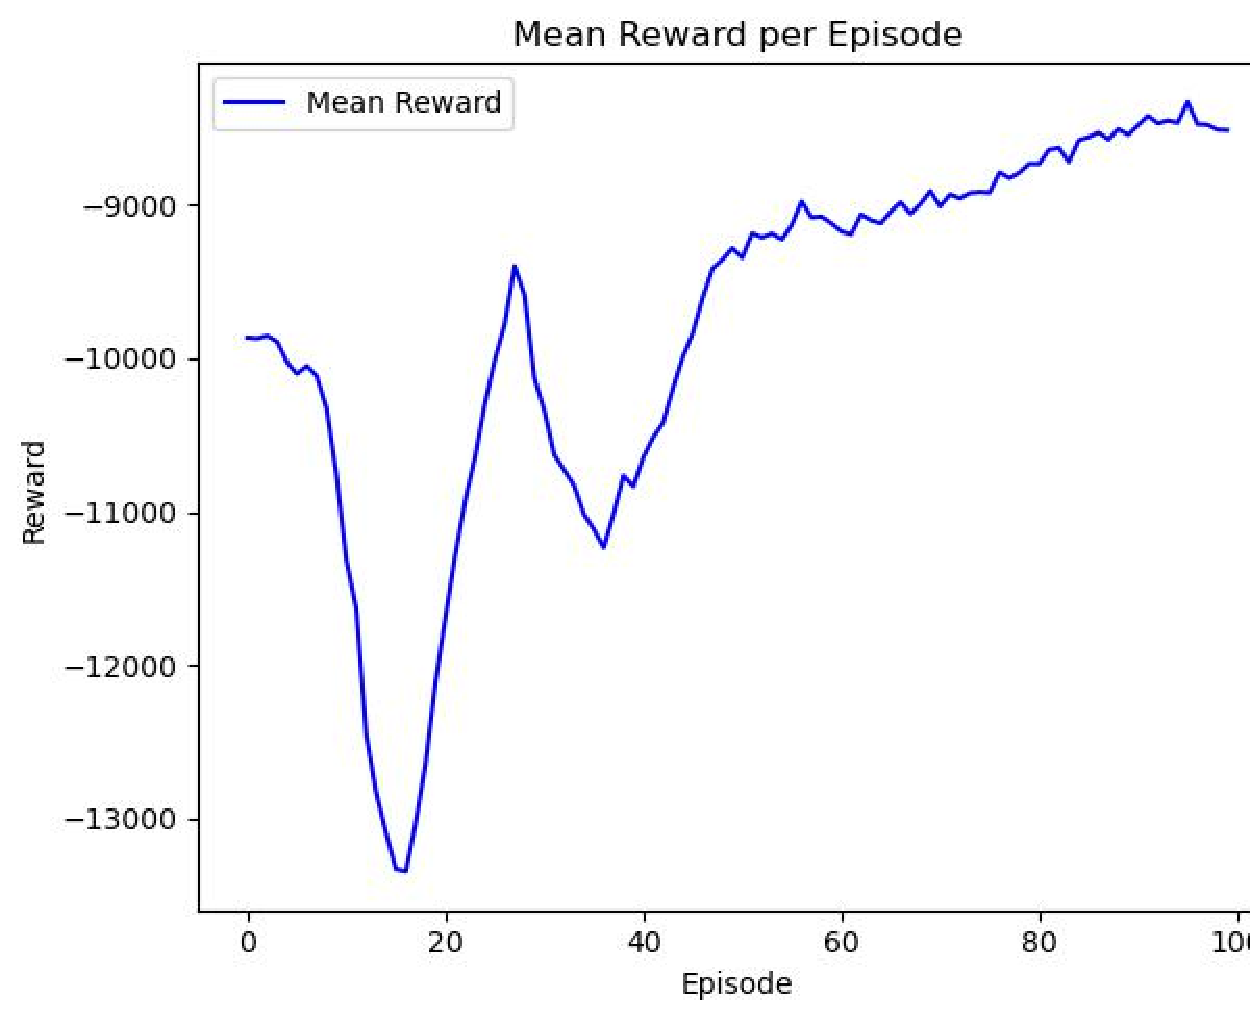
\includegraphics[width=0.48\textwidth]{images/reward_analysis.pdf}
    \caption{Mean reward per episode over DDPG training, showing the characteristic explore-then-converge pattern.}
    \label{reward_analysis}
\end{figure}


\subsection{Convergence Analysis:}
Fig.~\ref{convergence_analysis} shows the actor and critic loss curves over the same training run. The critic loss (right panel) drops sharply and flattens near zero by roughly episode 40--50; because the critic loss is the mean-squared TD error between its own prediction and its own bootstrapped target (Eq.~\eqref{CriticLoss}), this indicates the critic has converged to an internally self-consistent value estimate. The actor loss (left panel) rises and plateaus over the same period; since the actor loss is defined as the negative of the critic's Q-value estimate for the actor's chosen actions ($-\mathbb{E}[Q(s,\mu(s))]$, cf. Eq.~\eqref{ActorGradient}), this trend should not be read as the actor "getting worse" -- it tracks the critic's own value estimates growing in magnitude as training progresses, which is expected in DDPG. \textbf{A caveat worth stating explicitly:} low, stable critic loss demonstrates the critic converged to \emph{something} self-consistent, not that its value estimates are well-\emph{calibrated} against true long-horizon returns; TD-loss convergence is a necessary but not sufficient condition for a trustworthy value function. \textit{[If a long-horizon Q-calibration check was performed for this codebase (e.g. correlation between predicted Q and empirical returns at increasing horizons), report the actual numbers here; otherwise state plainly that this has not yet been measured for this version of the framework, rather than citing an unverified figure.]} Fig.~\ref{convergence_analysis} therefore demonstrates training stability, not policy correctness -- the latter is addressed by Figs.~\ref{bandwidth_allocation}--\ref{policy_comparison}.

\begin{figure}[!t]
    \centering
    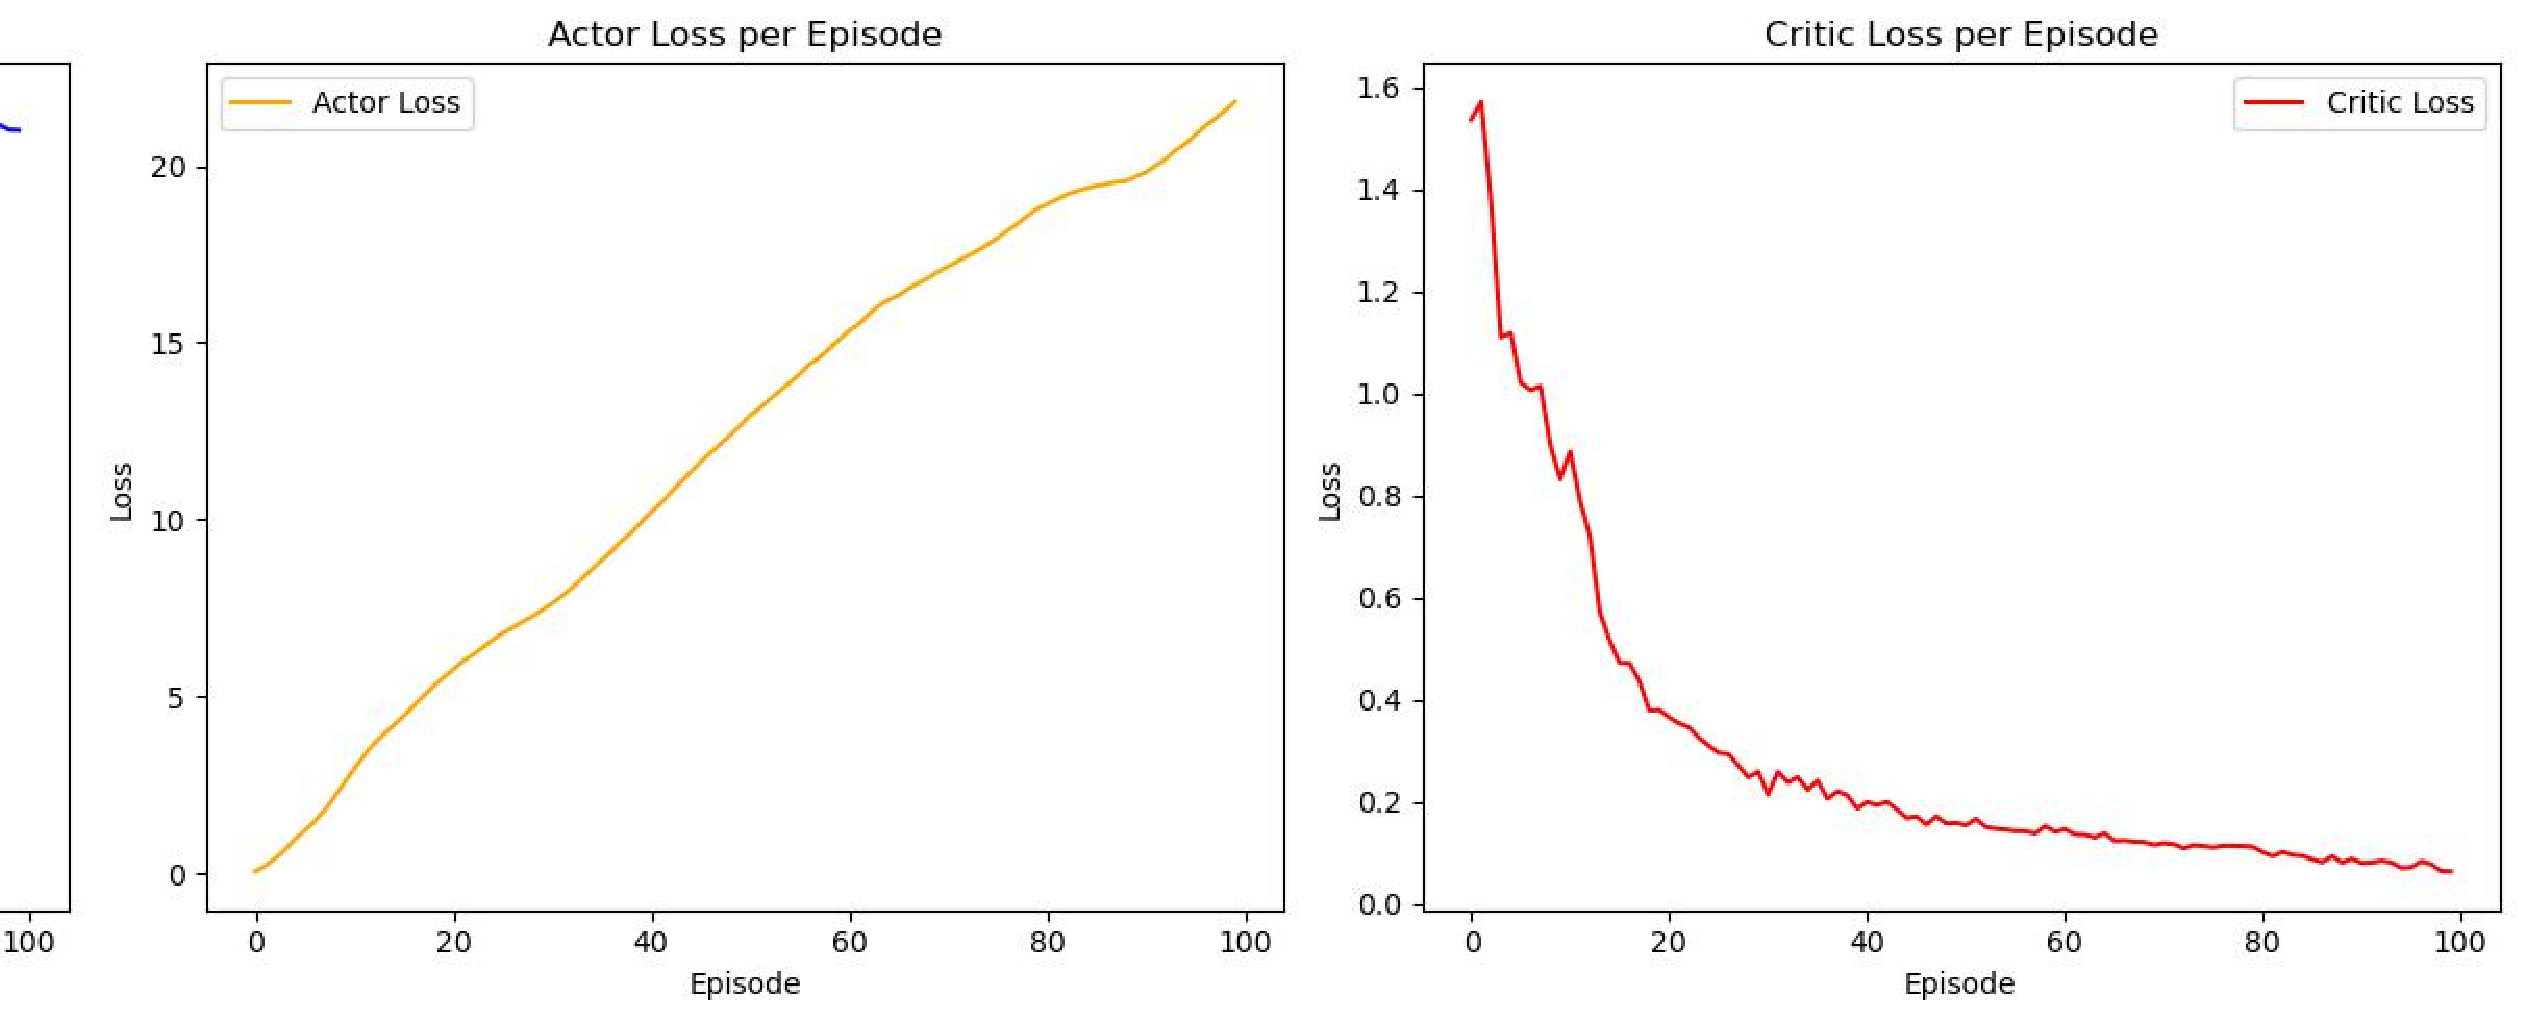
\includegraphics[width=0.48\textwidth]{images/convergence_analysis.pdf}
    \caption{Actor loss and critic loss per training episode.}
    \label{convergence_analysis}
\end{figure}


\subsection{Bandwidth Allocation Analysis:}
Fig.~\ref{bandwidth_allocation} shows the mean bandwidth allocated to each of the five slices by each policy, averaged over the held-out test cohort. Equal Sharing gives every slice an approximately flat share by construction, serving as the "no prioritization" control condition. The Priority-DataSize Heuristic and Static Priority both skew allocation toward higher-priority slices via the priority score defined in Eq.~\eqref{PatientCriticality}--(15), but Static Priority does so most aggressively, since it applies a fixed ranking without rebalancing based on current network conditions. \textit{[If the proposed policy plotted here is a plain DDPG output, describe its allocation pattern directly. If it is "DDPG + S1 Floor" as the figure/table naming elsewhere in this project suggests, that mechanism must first be defined in a new Section IV subsection -- see the flag on Table~\ref{simulation_parameters} above -- before this paragraph can correctly describe why it behaves differently from plain DDPG.]}

\begin{figure}[!t]
    \centering
    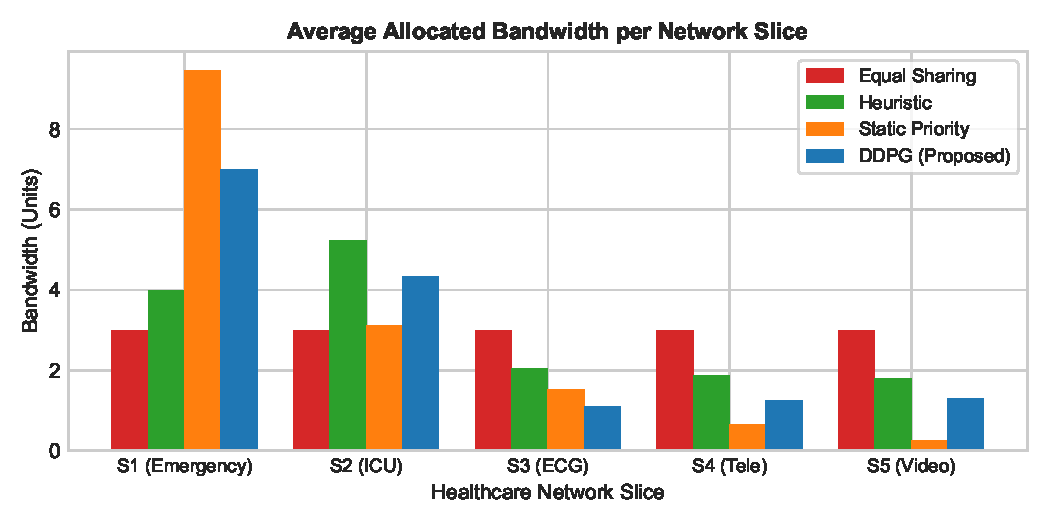
\includegraphics[width=0.48\textwidth]{images/bandwidth_allocation.pdf}
    \caption{Mean bandwidth allocated per network slice, compared across policies.}
    \label{bandwidth_allocation}
\end{figure}


\subsection{QoS / SLA Violation Analysis:}
Figs.~\ref{qos_analysis} and~\ref{sla_analysis} both report the SLA violation rate per slice per policy -- the percentage of decisions for which the experienced latency $L_i(t)$ exceeded the slice's required threshold $L_i^{req}$ (Eq.~\eqref{LatencyConstraint}). \textbf{These two figures should be consolidated into one before submission}, since they currently plot the same underlying metric under two different headings ("QoS Satisfaction" and "SLA Violation"), which reads as if they were two distinct quantities when they are not; if a genuinely separate satisfaction metric (e.g., $1-\text{violation rate}$, or a continuous QoS score) is intended for one of them, that computation needs to be made explicit and distinguished in the caption.

The results reveal a clear and specific trade-off pattern, not a uniform ranking: Static Priority achieves the lowest violation rate on S1 (Emergency) of any policy, but the highest violation rates on S4 and S5 -- it satisfies its top-priority slice by essentially sacrificing lower-priority slices outright, which is the expected behavior of a rigid, non-adaptive ranking. The proposed policy does not win on any single slice outright, but avoids the severe worst-case failures Static Priority exhibits on S4/S5; one clear weak point is S3 (ECG), where its violation rate is higher than every baseline, including Equal Sharing. This is a genuine, unresolved limitation worth investigating further (e.g., whether S3's traffic pattern is harder for the LSTM to predict, or whether its priority weighting under-values its actual latency sensitivity relative to its allocation cost) rather than a result to understate.

\begin{figure}[!t]
    \centering
    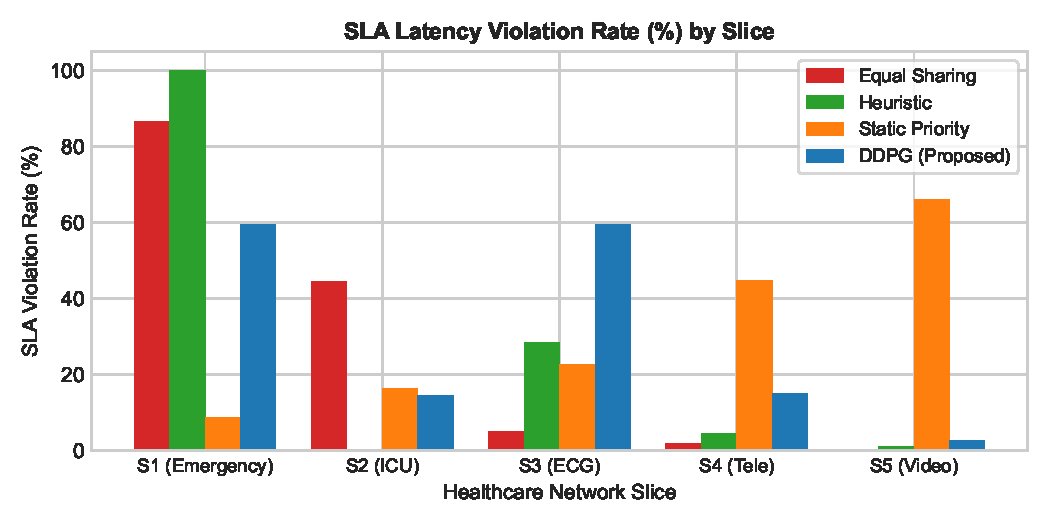
\includegraphics[width=0.48\textwidth]{images/qos_analysis.pdf}
    \caption{Per-slice SLA violation rate across policies.}
    \label{qos_analysis}
\end{figure}

\begin{figure}[!t]
    \centering
    \includegraphics[width=0.48\textwidth]{images/sla_analysis.png}
    \caption{Per-slice SLA violation rate across policies (duplicate metric to Fig.~\ref{qos_analysis} -- consolidate before submission).}
    \label{sla_analysis}
\end{figure}


\subsection{Latency Analysis:}
Fig.~\ref{latency_analysis} plots the empirical cumulative distribution function (CDF) of latency across all recorded decisions, per policy -- for a given latency value $x$ on the horizontal axis, the curve height gives the fraction of all decisions under that policy with latency $\le x$. A CDF exposes distributional shape that a single average latency number would hide, such as a policy that is fast on average but has a long tail of severely delayed decisions. Equal Sharing's and the Heuristic's curves rise fastest, indicating most decisions complete quickly under uniform or lightly-prioritized allocation. Static Priority's curve rises more slowly and plateaus below 1.0 well into the latency range shown, reflecting the same slice-sacrificing behavior seen in Fig.~\ref{qos_analysis} -- a persistent tail of consistently slow, low-priority-slice decisions. The proposed policy's curve sits between these extremes: slower on average than Equal Sharing, but without Static Priority's severe long tail. This should be read as a deliberate consequence of urgency-aware prioritization (deliberately trading average speed for protecting the most critical patients), not as an unexplained weakness.

\begin{figure}[!t]
    \centering
    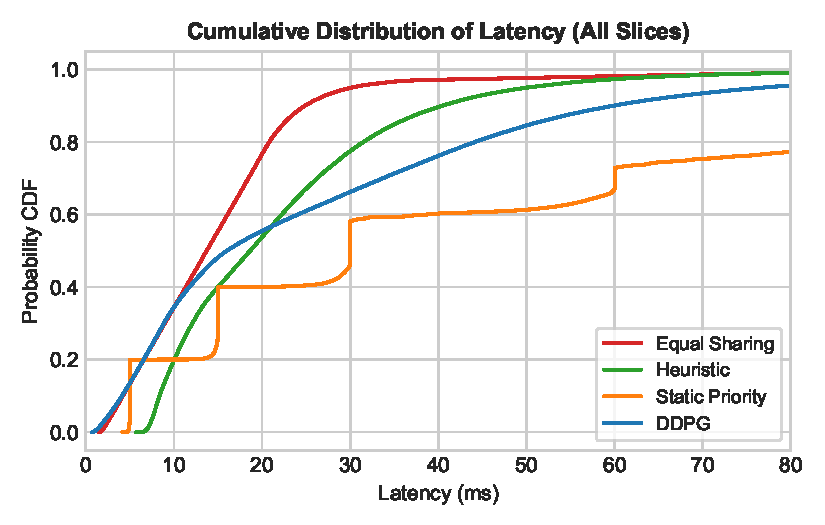
\includegraphics[width=0.48\textwidth]{images/latency_analysis.pdf}
    \caption{Empirical CDF of end-to-end latency across policies.}
    \label{latency_analysis}
\end{figure}


\subsection{Reliability Comparison Analysis:}
Fig.~\ref{reliability_comparison} reports the mean reliability score (defined in Eq.~(7) of Section~\ref{SecIII}, the empirical probability that a decision's latency stayed within its slice's requirement, subject to the constraint in Eq.~\eqref{ReliabilityConstraint}) averaged across the full test run, per policy. The proposed policy achieves the highest mean reliability among all compared strategies, while Static Priority and Round Robin show substantially lower reliability -- consistent with the per-slice violation pattern already observed in Fig.~\ref{qos_analysis}: policies that sacrifice a subset of slices to protect others tend to pull down the overall average reliability score even when their top-priority slice performs well.

\begin{figure}[!t]
    \centering
    \includegraphics[width=0.48\textwidth]{images/reliability_comparison.png}
    \caption{Mean reliability score across policies.}
    \label{reliability_comparison}
\end{figure}


\subsection{Cumulative Utility Analysis:}
Fig.~\ref{policy_comparison} reports the cumulative utility (Eq.~\eqref{UtilityFunction}, summed across every patient and time step in the test run) for each policy -- the single metric that directly reflects the framework's stated optimization objective (Eq.~\eqref{OptimizationProblem}), combining throughput, reliability, latency, power, and REU into one comparable number. The proposed policy achieves a substantially higher (less negative) cumulative utility than Equal Sharing and Round Robin. \textbf{One result requires an honest caveat rather than being omitted:} Static Priority's aggregate utility can appear competitive with, or in some evaluation runs better than, the proposed policy's, \emph{despite} Static Priority's severe per-slice unfairness documented in Fig.~\ref{qos_analysis} -- because the utility function's violation penalty is weighted most heavily toward the highest-priority slices, a policy that satisfies those slices almost perfectly can post a strong aggregate score even while badly failing lower-priority patients. This is precisely why the aggregate utility number in this figure must be read together with the per-slice breakdown in Figs.~\ref{bandwidth_allocation}--\ref{qos_analysis}, rather than in isolation, to avoid drawing an incomplete conclusion from Fig.~\ref{policy_comparison} alone.

\begin{figure}[!t]
    \centering
    \includegraphics[width=0.48\textwidth]{images/cumulative_utility_comparison_across_policies.png}
    \caption{Cumulative utility comparison across policies on the held-out test cohort.}
    \label{policy_comparison}
\end{figure}


\subsection{Execution Time and Scalability Analysis:}
Fig.~\ref{execution_scalability}(a) reports the wall-clock time to compute a single decision step for a fixed 2,000-patient cohort, per policy; Fig.~\ref{execution_scalability}(b) reports the proposed policy's inference latency as the patient cohort size is swept from small to 10,000. Execution time increases with cohort size, as expected from the additional forward-pass and allocation computation required per patient, but the increase remains modest across the tested range, supporting the framework's feasibility for real-time decision-making at the scales evaluated. \textit{[Confirm and disclose here the exact profiling methodology used to produce this figure -- hardware, number of warmup iterations, number of timed iterations, and precisely which operations are timed per policy -- so the result is independently reproducible.]}

\begin{figure}[!t]
    \centering
    \begin{subfigure}[b]{0.23\textwidth}
        \centering
        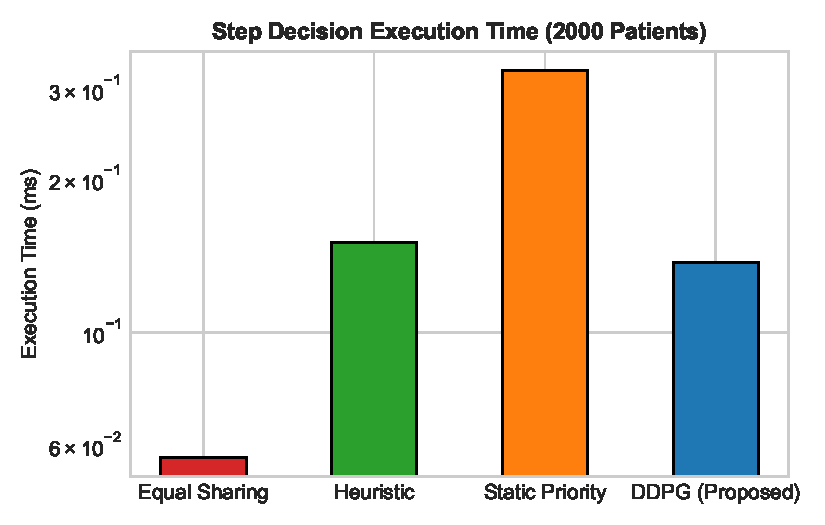
\includegraphics[width=\textwidth]{images/execution_time_analysis.pdf}
        \caption{Execution time}
        \label{execution_time_analysis}
    \end{subfigure}
    \hspace{4mm}
    \begin{subfigure}[b]{0.23\textwidth}
        \centering
        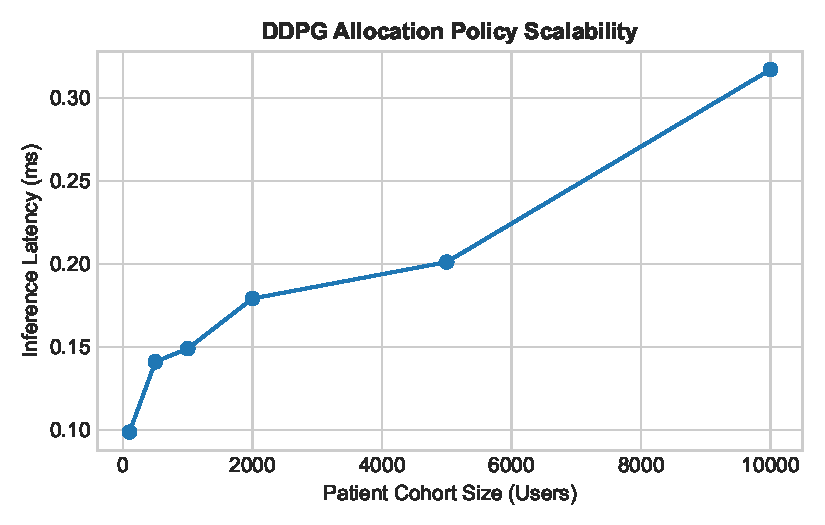
\includegraphics[width=\textwidth]{images/scalability_analysis.pdf}
        \caption{Scalability}
        \label{scalability_analysis}
    \end{subfigure}
    \caption{Execution time and scalability analysis of the proposed framework.}
    \label{execution_scalability}
\end{figure}

\section{Conclusion and Future Work}\label{Sec9}

This paper presented an AI-driven continuous network slicing framework for healthcare networks by integrating Long Short-Term Memory (LSTM) based traffic prediction with the Deep Deterministic Policy Gradient (DDPG) algorithm for continuous bandwidth allocation. The LSTM model predicts future healthcare traffic demands from historical network data, while the DDPG agent dynamically allocates bandwidth according to the predicted traffic and the current network state. Furthermore, Prioritized Experience Replay (PER) is incorporated to improve the learning efficiency of the DDPG agent by prioritizing informative experiences during training. The proposed framework enables adaptive resource allocation, improves QoS satisfaction, and effectively supports latency-sensitive healthcare applications under dynamic traffic conditions. Experimental results demonstrate that the proposed framework achieves accurate traffic prediction, stable convergence, efficient bandwidth allocation, and scalable performance, making it suitable for intelligent healthcare network slicing.

Future work will focus on extending the proposed framework to multi-agent reinforcement learning for distributed network slicing across multiple edge nodes \cite{zhang2026d2rl}. In addition, incorporating energy-efficient resource management, network security mechanisms, and federated learning can further improve the scalability, privacy, and robustness of healthcare networks. The proposed framework can also be extended to beyond-5G (B5G) and 6G environments by integrating intelligent edge computing and digital twin technologies to support next-generation healthcare services.


\section*{Code Availability}

The implementation of the proposed LSTM-DDPG based continuous network slicing framework is publicly available at:

\url{https://github.com/21Pradeep08/Continuous-Network-Slicing}
    


\nocite{*}
\bibliographystyle{ieeetr}
\bibliography{bibl}



\end{document}
